\documentclass[preprint,12pt]{elsarticle}

%% Acta Astronautica (Elsevier) -- elsarticle class. Sectionized layout:
%% sections/01..08_*.tex combined here; References LAST. Compile:
%%   pdflatex -interaction=nonstopmode main && bibtex main &&
%%   pdflatex -interaction=nonstopmode main &&
%%   pdflatex -interaction=nonstopmode main

\graphicspath{{../figures/}{../supplementary/}}

\usepackage{amsmath,amssymb}
\usepackage{booktabs}
\usepackage{siunitx}
\usepackage[hidelinks]{hyperref}

\journal{Acta Astronautica}

\begin{document}

\begin{frontmatter}

\title{Robust shape optimization of a ballistic entry capsule under
entry-condition and aerodynamic model-form uncertainty}

\author[a]{Md Jaminur Rahman Khalid\corref{cor1}}
\ead{mrjkhalid5@gmail.com}
\cortext[cor1]{Corresponding author.}
\author[a]{Mahbubul Alam}
\affiliation[a]{organization={Department of Mechanical Engineering,
                Chittagong University of Engineering and Technology},
                city={Chattogram},
                postcode={4349},
                country={Bangladesh}}

\begin{abstract}
Shape optimization of entry capsules is conventionally deterministic: one
nominal entry state, one aerodynamic model. We test this practice by
comparing deterministic and robust formulations of a three-objective
capsule problem---maximize volumetric efficiency, minimize integrated
heat load, maximize range---on one local-inclination aerothermal model,
component-validated against Apollo data, and common Gaussian-process
surrogates, under entry-state dispersion combined with aerodynamic
model-form uncertainty sized from validation residuals. At matched
expected performance, robust designs improve on their matched
deterministic counterparts in 98.1\% of 5{,}371 matched pairs, with a
median heat-load-dispersion reduction of 27.5\% at pair level and 35.0\%
against the lowest-$\sigma$ robust design available at matched
performance --- results stable across optimizer seeds and a factor-three
range of dispersion assumptions. The
deterministic front conceals shoulder-heating exceedance probabilities up
to 10\%, confirmed at 9.7\% by Monte-Carlo simulation, and its optimum
exploits a surrogate extrapolation blind spot, overpredicting nominal
range 3.5-fold. Within the studied design space, heat-load dispersion has
a geometry-insensitive floor of about
\SI{16}{\mega\joule\per\square\metre} (coefficient of variation 20\%),
set by the flight-path-angle dispersion rather than shape.
\end{abstract}

\begin{keyword}
capsule aerothermodynamics \sep shape optimization \sep robust design \sep
uncertainty quantification \sep Gaussian process surrogate \sep
multi-objective optimization
\end{keyword}

\end{frontmatter}

%======================================================================
% 1. INTRODUCTION
%======================================================================
\section{Introduction}
\label{sec:intro}

The external geometry of a ballistic entry capsule settles most of its entry
performance before a single trajectory is flown. Nose radius, shoulder radius
and afterbody cone half-angle set the force coefficients and the trim and
stability characteristics, and through them the integrated heat load, the
attainable ground range and the enclosed payload volume. Shape optimization
therefore resolves a three-way trade between thermal load, mobility and
volumetric efficiency, under limits on peak heating, deceleration and static
stability. In most of the literature this trade is resolved deterministically:
one nominal entry state and one aerodynamic model are assumed, and dispersion
is absorbed downstream by margins in the thermal-protection and guidance
design, without feedback into the shape itself.

Deterministic capsule shape optimization is well explored. Dirkx and Mooij
\cite{dirkx2014,dirkx2017entry} optimize capsule shapes with
local-inclination aerothermal models and evolutionary algorithms; the
present simulation chain descends from that work. Related aerodynamic
capsule designs and parameterized-shape optimizations are reported by Chen
et al.\ \cite{chen2015}, and the surrogate-modelling toolbox behind such
workflows \cite{forrester2008surrogate} rests on the
design-and-analysis-of-computer-experiments literature
\cite{sacks1989,jones1998}.
The uncertainty-aware literature is thinner. Ridolfi et al.\
\cite{ridolfi2012robust} made a multi-disciplinary capsule optimization
robust to uncertainty in design parameters and mission conditions, and
Ghaedamini Harouni and Hashemi Mehneh \cite{hashemi2019capsule} solved a
robust multi-objective capsule shape problem --- maximizing volumetric
efficiency among the objectives --- with adaptive Monte-Carlo inner loops,
reporting constraint satisfaction at a 99.8\% confidence level. Both
establish that robustness can be enforced on capsule shape design; neither
compares the robust result against a deterministic baseline solved on the
same physics, which is what isolates the effect of the formulation itself.
The general theory of robust optimization \cite{beyer2007robust} and the
reliability-based tradition surveyed by Valdebenito and Schu\"eller
\cite{valdebenito2010} flag two recurring obstacles that are visible in
these applications: the cost of the inner uncertainty propagation, and the
weak evidence base of the uncertainty model itself.

For capsule shape design specifically, three gaps remain. First, the
uncertainty bands entering robust or reliability-based formulations are
usually assumed: entry-state dispersions are inherited from targeting
budgets, and aerodynamic model-form error is assigned a round percentage with
little justification. Second, deterministic and robust formulations are
rarely solved on the same validated physics, so any reported ``benefit of
robustness'' mixes the formulation change with model and solver differences.
Third, the cost of ignoring uncertainty is seldom quantified, and even less
often verified: what a deterministic front hides in constraint-exceedance
probability and objective dispersion is typically not measured against the
true model.

This paper closes the three gaps with a controlled comparison on a single
simulation chain. The uncertainty model is evidence-based: entry-state
dispersion (flight-path angle, entry speed) is combined with a multiplicative
aerodynamic model-form uncertainty whose 5\% standard deviation is sized from
the residuals of a validation campaign against Apollo wind-tunnel and flight
data, not chosen for convenience. Deterministic and robust formulations of
the same three-objective problem are then solved on the same Gaussian-process
surrogates, evaluated by a common-random-number moment engine so that the two
fronts are directly comparable, and the deterministic front is additionally
audited under the full uncertainty model. The comparison is quantified rather
than asserted: at matched expected performance, robust designs cut the
standard deviation of integrated heat load in 98.1\% of 5{,}371 design pairs
(pair-level median 27.5\%; 35.0\% against the robust front's
$\sigma$-envelope at matched performance), while the deterministic front
conceals
shoulder-heating exceedance probabilities up to 10\%, confirmed at 9.7\% by
Monte-Carlo simulation of the full model. An irreducible dispersion floor of
\SI{16}{\mega\joule\per\square\metre} (coefficient of variation about 20\%)
bounds both fronts and is set by the flight-path-angle dispersion, not by
geometry. Finally, selected designs are verified against the trajectory
simulator itself, 1{,}500 runs in total; the same exercise exposes a
systematic bias of the mixture surrogate in predicted range, which we
disclose and bound.

Section~\ref{sec:model} describes the vehicle model and its validation.
Sections~\ref{sec:surrogate} and \ref{sec:formulation} present the
uncertainty model, the surrogate construction and its accuracy gate, and the
two design formulations. Section~\ref{sec:results} reports the front
comparison, Section~\ref{sec:verification} the Monte-Carlo verification, and
Sections~\ref{sec:discussion} and \ref{sec:conclusions} the discussion and
conclusions.

%======================================================================
% 2. ENTRY-VEHICLE MODEL AND VALIDATION
%======================================================================
\section{Entry-vehicle model and validation}
\label{sec:model}

\subsection{Geometry and parameterization}
\label{sec:geometry}

The vehicle is an axisymmetric capsule consisting of a spherical-section
forebody, a toroidal shoulder and a conical afterbody frustum
\cite{dirkx2017entry}. Three shape parameters are free: the nose radius
$R_n$, the shoulder radius $R_s$ and the afterbody cone half-angle
$\theta_c$. The maximum body radius ($R_m=\SI{2}{\metre}$) and the frustum
length ($L_c=\SI{2}{\metre}$) are held fixed, so the design space is
three-dimensional; Table~\ref{tab:bounds} lists the bounds. In the
optimizers the three variables are normalized to $[0,1]$.

Each shape carries its own mass through the Apollo-derived
constant-density model of \cite{dirkx2017entry}: the Apollo command module
($m=\SI{5470}{\kilogram}$, $V=\SI{20.02}{\cubic\metre}$) implies
$\rho=\SI{273.29}{\kilogram\per\cubic\metre}$, and $m=\rho V(\mathbf{x})$.
The centre-of-gravity placement follows the same Apollo-based offset model
and is not optimized. The first objective, volumetric efficiency
\begin{equation}
\eta_V \;=\; \frac{6\sqrt{\pi}\,V}{S^{3/2}} \;\in\; (0,1],
\label{eq:etav}
\end{equation}
equals unity for a sphere and rewards enclosed volume per wetted area; it
is an exact geometric quantity, evaluated from the shape and never
surrogated.

\begin{table}[htbp]
\centering
\caption{Design variables and fixed geometry.}
\label{tab:bounds}
\begin{tabular}{lccl}
\toprule
parameter & symbol & bounds & role \\
\midrule
nose radius            & $R_n$    & $3$--$7$ \si{\metre}          & free \\
shoulder radius        & $R_s$    & $0.02$--$0.4$ \si{\metre}     & free \\
afterbody half-angle   & $\theta_c$ & $5$--$60$ \si{\degree}      & free \\
max.\ body radius      & $R_m$    & $2$ \si{\metre} (fixed)       & fixed \\
afterbody length       & $L_c$    & $2$ \si{\metre} (fixed)       & fixed \\
\bottomrule
\end{tabular}
\end{table}

%% TODO figure (to build; thesis Fig 3.5 as template):
%% \begin{figure}[htbp]
%%   \centering\includegraphics[width=\linewidth]{fig_geometry_schematic}
%%   \caption{Capsule parameterization: spherical-section forebody
%%     (Rn), shoulder radius (Rs), afterbody cone half-angle (theta_c);
%%     local surface normal shown for the local-inclination method.}
%%   \label{fig:geometry}
%% \end{figure}

\subsection{Aerothermal model}
\label{sec:aero}

The atmosphere follows the U.S.\ Standard Atmosphere 1976 with the tabulated
86--120~km extension, interpolated between nodes \cite{us1976atmosphere};
above the homopause density is interpolated directly rather than recovered
from the gas law. Surface pressures come from a local-inclination method
\cite{dirkx2017entry,hirschel2009}: modified Newtonian on the windward
spherical nose,
an exact Taylor--Maccoll tangent-cone solution on the afterbody cone
(saturating to the Newtonian level beyond shock detachment), and
Prandtl--Meyer expansion on lee surfaces, with the cone and prism laws
Mach-blended over $M=5$--$12$ for continuity. Integrating the local
coefficients over the meridional contour yields $C_D$, $C_L$ and $C_m$
databases on a grid of $M\in[3,30]$ (ten nodes) and
$\alpha\in[-5^\circ,35^\circ]$ (41 nodes); bivariate interpolation supplies
forces and moments in flight. The trim angle of attack solves $C_m=0$ at
each Mach number, and the trajectory flies at trim.

Stagnation-point convective heating uses the Sutton--Graves form of the
$\sqrt{\rho}\,V^3$ correlation \cite{sutton1971}
with the effective nose radius $R_{\mathrm{eff}}$ of Zoby and Sullivan
\cite{zoby1965heating}, read from their chart for the actual
$(R_m/R_n,\,R_s/R_m)$ combination; the in-code chart reproduces the
published curves to within 1.4\% over the design space. Shoulder heating is
taken as a correlated fraction of the stagnation value through a linear
relation in Mach number, angle of attack, $R_s/R_m$ and the nose-sphere
half-angle, fitted to wind-tunnel measurements of the shoulder-to-stagnation
ratio; the fit reproduces the source ratios to within 10.2\% and inherits
their trends (rising with $\alpha$, falling with $R_s$). A cold wall
($T_w/T_{aw}=0$) is assumed throughout.

\subsection{Trajectory simulation}
\label{sec:traj}

Entry is propagated with a point-mass three-degree-of-freedom model over a
spherical, rotating Earth, in the ballistic-entry tradition of Allen and
Eggers \cite{allen1958} as formalized for entry mechanics by Vinh et al.\
\cite{vinh1980}. The state is
$(h,V,\gamma,\varphi,\lambda,\chi,\sigma)$; the bank angle $\sigma$ is a
propagated seventh state that tracks the no-skip bank command of
\cite{dirkx2017entry} through a first-order lag capped at
\SI{5}{\degree\per\s}, which removes the on/off chatter of the idealized
command and mirrors the finite roll rate of a real vehicle. The modulation
is active only while $0<\cos\sigma<1$; outside that band the vehicle flies
full lift-up. Integration uses an adaptive Runge--Kutta scheme and
terminates at $M=3$, with a horizon of $t_{\max}=\SI{14400}{\s}$ (the
horizon was raised from an initial 7{,}200~s during data-quality auditing;
Section~\ref{sec:doe}).

Each run returns five quantities: the integrated stagnation heat load
$Q_s=\int q_{\mathrm{stag}}\,dt$; the range $sg$, defined as the
great-circle distance between the entry-interface position and the final
position (a lower bound on ground-track length, with a physical maximum of
$\pi R_{\oplus}\approx\SI{20015}{\kilo\metre}$); the peak stagnation and
shoulder heat fluxes; and the peak load factor. The load-factor metric is
drag-based, $n_D=D/(mg)$; the total-force definition
$n=\sqrt{D^2+L^2}/(mg)=n_D\sqrt{1+(L/D)^2}$ exceeds it by 4--5\% at capsule
lift-to-drag ratios, and both are reported where the distinction matters.

\subsection{Validation against reference data}
\label{sec:validation}

The chain was validated layer by layer against Dirkx and Mooij
\cite{dirkx2017entry}, whose reference figures were digitized (per-subpanel
calibration; tracing artifacts removed by a documented filter, with all
verdicts re-checked for stability); the full audit, including the
reference-data forensics summarized below, is reproduced in
Appendix~\ref{app:validation}. Component-level verification against
analytic benchmarks (Taylor--Maccoll against exact cone solutions,
Prandtl--Meyer against published anchor angles, atmosphere against
standard tables) precedes any comparison with the reference mission, so
equation and implementation errors are separated from mission-level
agreement throughout. The atmosphere reproduces the standard
anchor values to $2\times10^{-5}$ relative. The surface-pressure laws match
the book's correlation charts to within 0.026~$C_p$ (modified Newtonian) and
0.061~$C_p$ (tangent-cone core, $M=3$, against a 0.065 band attributable to
the documented beyond-detachment treatment). The core aerodynamic check
compares Apollo force coefficients at $M=3$ and $M=10$ against wind-tunnel
data as re-plotted by Dirkx and Mooij (originally from the stability test
campaign of NASA TN D-3890 \cite{moseley1967d3890}, with the flight and
tunnel data bases of \cite{hillje1969apollo,moseley1969wind}): nine of nine
checks pass,
lift-to-drag ratio to within 0.029 absolute and the coefficient shapes to
within 0.015 after scale removal. The known over-prediction of
$C_D(\alpha\approx0)$ at $M=10$ inherent to local-inclination methods lands
at 1.610 against a wind-tunnel value of 1.523 --- between the tunnel and the
book's own implementation (1.704). The heating model reproduces the
Zoby--Sullivan chart to 1.4\%, the shoulder-ratio sources to 10.2\%, and the
computed trim angles match the reference trim curve to 0.33$^\circ$.

On the full Apollo entry case ($V_0=7.83$~km/s, $\gamma_0=-4^\circ$,
$m=4532$~kg, the reference initial conditions), the implementation
reproduces the published peak heat rate to 0.7\%; integrated heat load and
track length sit $+32\%$ and $+16\%$ above the reference table. The
end-to-end differences are bounded and attributed rather than resolved:
they concentrate in the guidance realization and in the reference data
themselves. Panel~(c) of the reference Fig.~7.17 plots $\dot{q}(M)$ and
$n(M)$ for one simulation; these quantities are algebraically coupled
independent of trajectory model, and the digitized pair violates that
identity by factors of 0.17--0.65, so the load-factor panel is not a valid
target --- and the reference table itself lies below every member of a
documented variant family of the bank law whose digitized $\dot{q}$ curve
runs above ours (Appendix~\ref{app:variants}). Within that family, peak
heat rate and track length are individually reproducible to 0.7\% and
$-1.1\%$, and no member reproduces the table and the panels
simultaneously; the family floor for integrated heat load is $+16\%$. The
deviations between the present implementation and the reference --- the
bank-rate limit, the Prandtl--Meyer lee treatment, the omission of base
pressure, the Mach-grid extension to 30, and the moment-reference and
load-factor conventions --- are each quantified in
Appendix~\ref{app:deviations}. In short, the model is
\emph{component-validated} at the percent level, with end-to-end
discrepancies against the single available reference case attributed to
specific, documented causes; the residual force-level model-form error is
what the uncertainty model of Section~\ref{sec:surrogate} represents.

Which of this paper's claims depend on that residual absolute accuracy is
therefore worth stating once, explicitly, as three claims of different
strength. (i)~\emph{The component models reproduce their analytical and
reference benchmarks}: supported at the percent level above. (ii)~\emph{The
complete simulator produces credible predictions for this entry
scenario}: partially supported --- peak heat rate reproduces the only
end-to-end reference to 0.7\%, while integrated heat load and track length
sit $+32\%$/$+16\%$ above a reference table that is itself internally
inconsistent; the discrepancies are bounded and attributed
(Appendix~\ref{app:validation}), not resolved. (iii)~\emph{The relative
comparison between the two formulations is reliable}: supported by
construction --- every comparison runs on one simulator, one surrogate,
and one common-random-number lens, so shared model error cancels to first
order --- and by simulator-level verification
(Section~\ref{sec:verification}). The paper's conclusions rest on (i)
and (iii); (ii) bounds the absolute meaning of objective values and of
the constraint-boundary positions (the 5-$g$ and heat-flux limits bind
against aerodynamics whose absolute level carries the attributed offset),
not the comparisons themselves. The sensitivity studies of
Sections~\ref{sec:surrogate} and \ref{sec:sens} additionally probe the
reported statistics against changes in the uncertainty model itself.

\begin{figure}[htbp]
\centering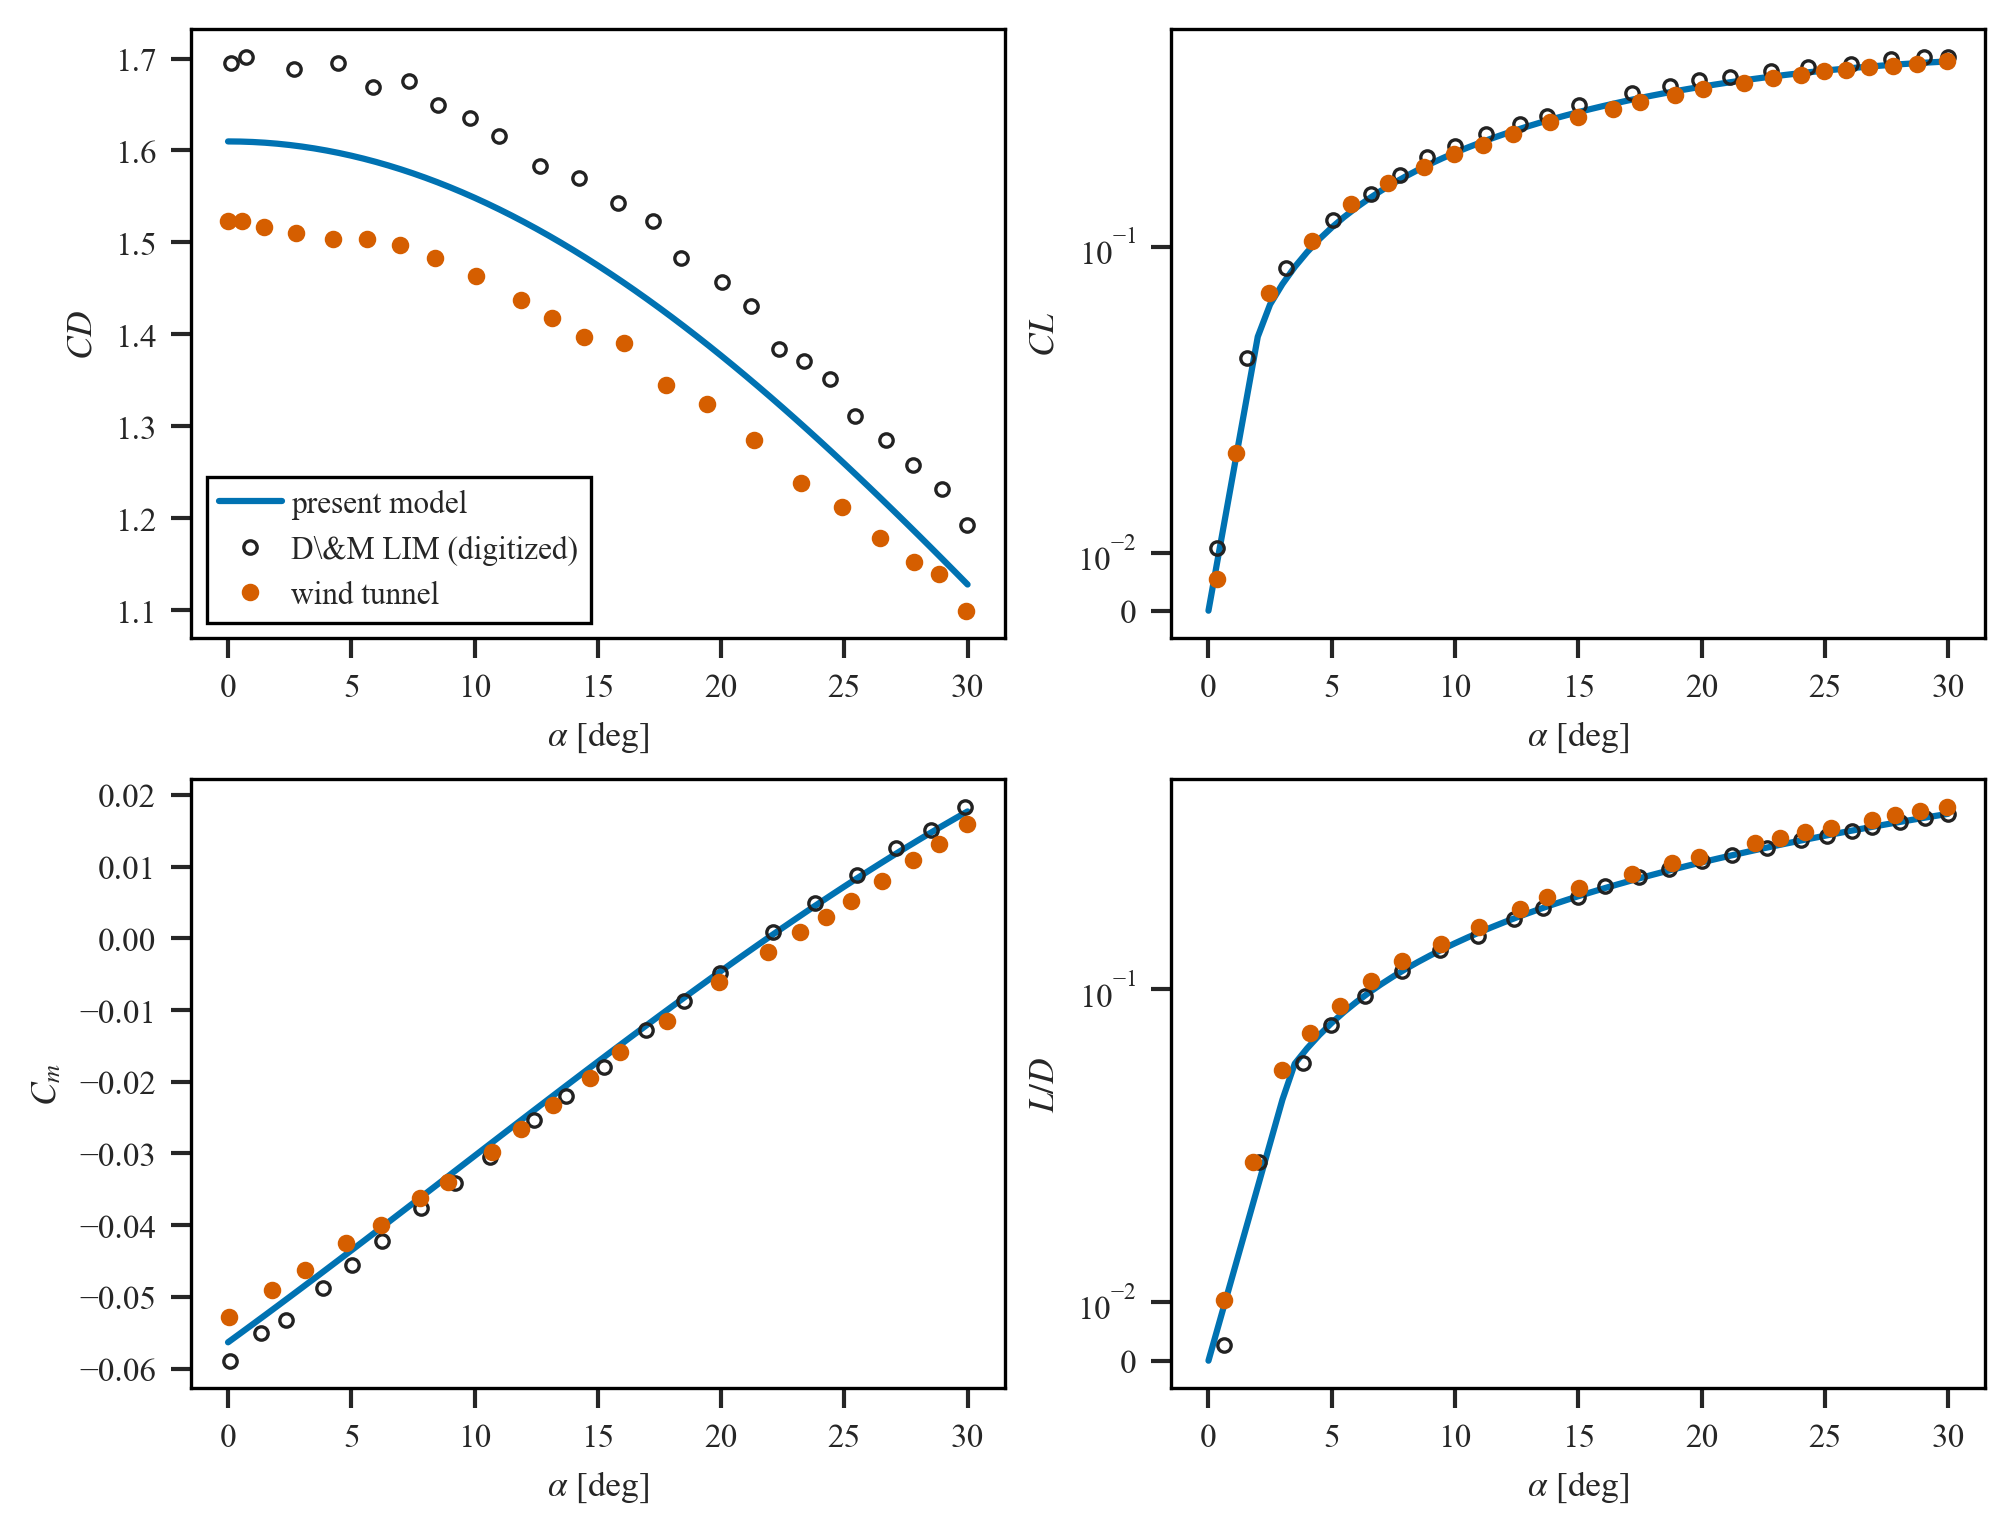
\includegraphics[width=\linewidth]{fig_validation_aero}
\caption{Apollo force coefficients at $M=10$: present local-inclination
  model (line), the digitized local-inclination curves of the reference
  (circles), and wind-tunnel data (crosses), in the present model's
  angle-of-attack sign convention. Lift-to-drag agrees to within 0.007
  absolute; the known local-inclination over-prediction of
  $C_D(\alpha\approx0)$ places the present model (1.610) between the
  tunnel (1.523) and the reference implementation (1.704). The $M=3$
  counterpart is Fig.~S2 (supplementary material).}
\label{fig:v2aero}
\end{figure}

\begin{figure}[htbp]
\centering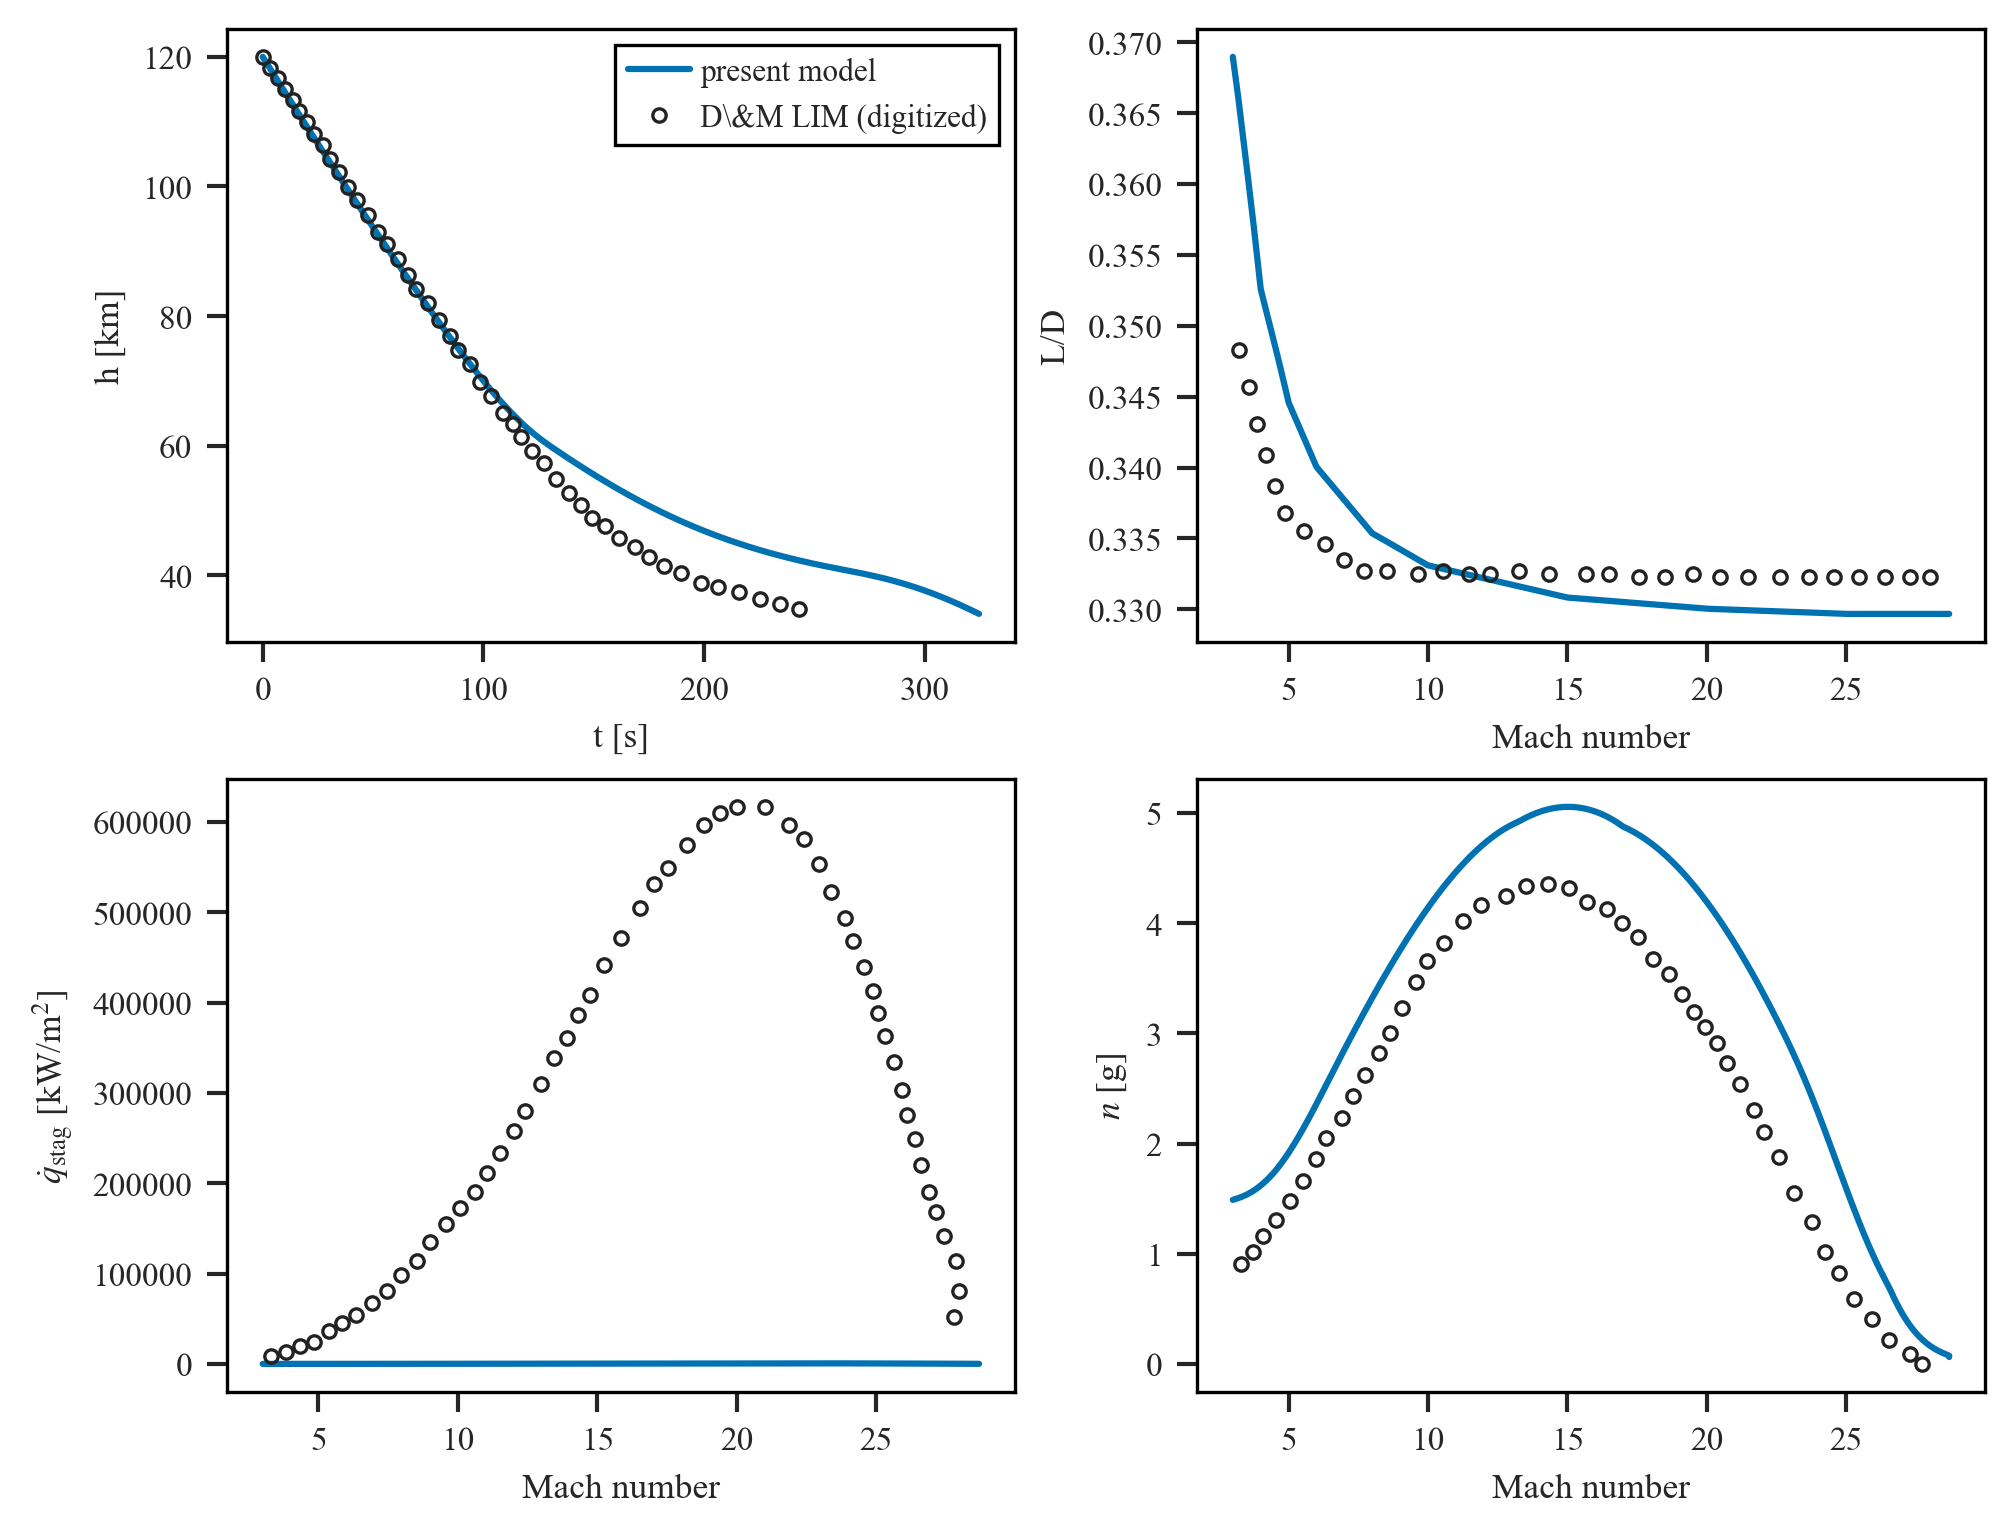
\includegraphics[width=\linewidth]{fig_validation_traj}
\caption{Apollo entry case ($V_0=7.83$~km/s, $\gamma_0=-4^\circ$,
  $m=4532$~kg): altitude, lift-to-drag ratio, stagnation heat rate, and
  load factor from the present model (lines) against the digitized
  reference profiles (circles). Peak heat rate reproduces the reference
  to 0.7\%; the load-factor panel is qualitative only, per the reference
  inconsistency documented in Appendix~\ref{app:identity}.}
\label{fig:v4traj}
\end{figure}

\begin{figure}[htbp]
\centering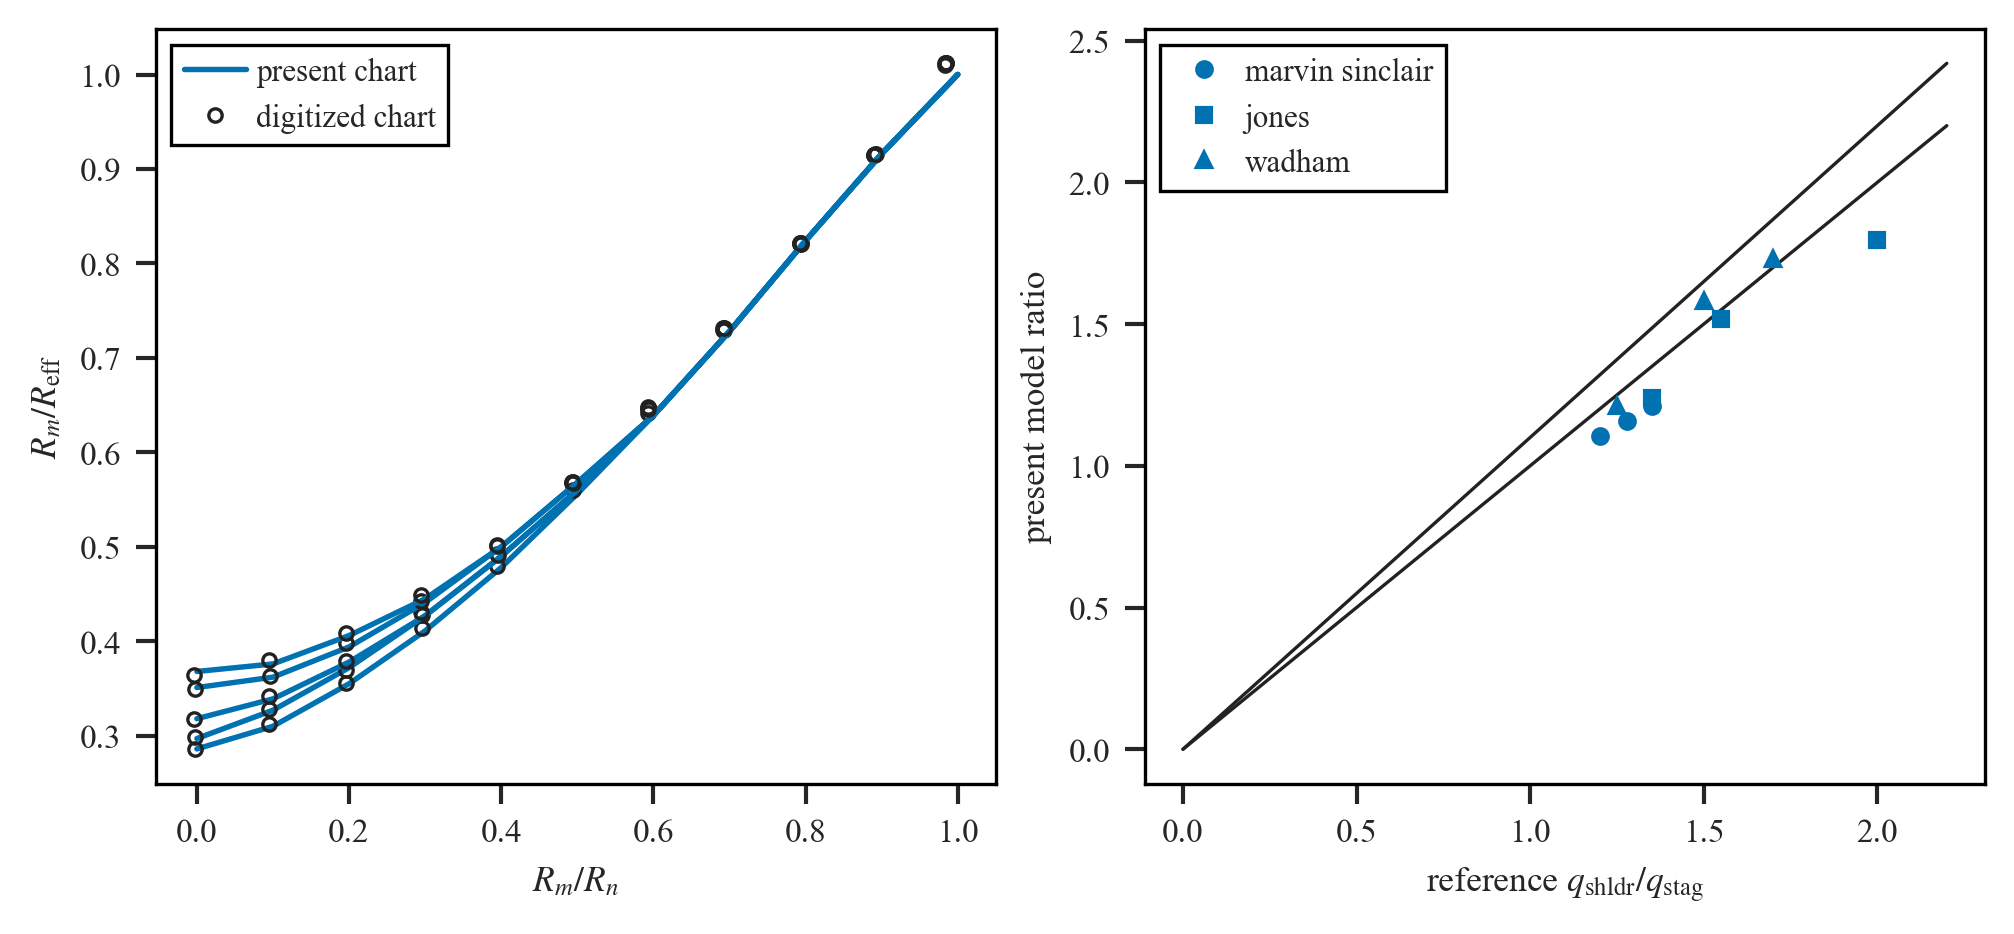
\includegraphics[width=\linewidth]{fig_validation_heating}
\caption{Heating-model validation. (a) Zoby--Sullivan effective
  nose-radius chart: present interpolation (lines) against the digitized
  chart (circles) for five shoulder-to-body radius ratios, agreement
  within 0.014 over the design-space region ($R_m/R_n\le0.7$). (b)
  Shoulder-to-stagnation heat-flux ratio: present correlation against
  the wind-tunnel source measurements, worst deviation 10.2\%.}
\label{fig:v3heat}
\end{figure}

%======================================================================
% 3. UNCERTAINTY MODEL AND SURROGATE CONSTRUCTION
%======================================================================
\section{Uncertainty model and surrogate construction}
\label{sec:surrogate}

\subsection{Uncertain variables}
\label{sec:uncertainty}

Four inputs are uncertain (Table~\ref{tab:uncert}). Two describe the
entry-interface state: the flight-path angle
$\gamma_0\sim\mathcal{N}(-2^\circ,\,0.5^\circ)$ and the entry speed
$V_0\sim\mathcal{N}(7830,\,50)$~m/s, the nominal values being those of the
underlying optimization case. The magnitudes --- half a degree on
flight-path angle, 0.6\% on speed --- are representative of
entry-interface targeting accuracy for guided lunar-return entries, but
they are assumptions, not measurements: Section~\ref{sec:sens} therefore
brackets $\sigma_{\gamma_0}$ over a factor of three, and every comparison
conclusion survives that range. Two represent aerodynamic model form:
multiplicative factors $k_{CD},k_{CL}\sim\mathcal{N}(1,\,0.05)$ applied to
the drag and lift interpolators. The factors perturb force magnitudes at
fixed trim (the trim angle comes from the unscaled moment), which isolates
force-level model error from trim prediction. All four are treated as
independent; sampling is by Latin hypercube through the inverse CDF.
Independence of the two scale factors is the weakest part of this
specification --- the fitted Mach-wise scale factors move together across
Mach --- and Section~\ref{sec:sens} therefore probes every headline
statistic against correlated scales, wider and narrower scale bands, and
alternative entry-state dispersions.

The 5\% band on $k_{CD}$ and $k_{CL}$ is sized from the validation
residuals of Section~\ref{sec:validation} rather than assumed.
Table~\ref{tab:calib} shows the calibration audit explicitly: for each
force coefficient at the two validation Mach numbers, the median scale
factor that best aligns the model with the digitized curves, its distance
from unity in units of the assumed $\sigma_k=0.05$, and the residual shape
error that remains after that scale is removed. Two features size the
model. First, the post-scale residuals are small: at most 0.013
(0.9--2.2\% of the coefficient magnitude) in three of the four
coefficient/Mach combinations, with $C_D$ at $M=3$ the outlier at 0.060
(4.4\%), the documented tangent-cone beyond-detachment case --- so a
multiplicative band of a few percent covers the residual error. Second,
the fitted scales are themselves Mach-structured: near 0.95 at $M=10$
($\approx1\sigma$) but 1.11 and 1.19 for $C_D$ and $C_L$ at $M=3$ (2.2
and 3.7$\sigma$). A single trajectory-constant Gaussian multiplier cannot
represent that structure exactly, and we do not claim it does: the 5\%
standard deviation covers the residual error comfortably and treats the
$M=3$ calibration bias --- which a trajectory-constant factor would
partially average over the entry Mach range --- as a tail event rather
than a central one. What protects the conclusions is that they do not
depend on this choice: Section~\ref{sec:sens} varies $\sigma_k$ by
$\pm40\%$, correlates the two factors, and brackets $\sigma_{\gamma_0}$ by
a factor of three, with every headline statistic moving within a few
percentage points. The uncertainty model is thus \emph{sized from}
validation evidence in a traceable sense --- an exercise in
calibration-informed uncertainty in the spirit of Kennedy and O'Hagan
\cite{kennedy2001} --- not calibrated in the strict sense of a fitted
posterior.

\begin{table}[htbp]
\centering
\caption{Calibration audit of the aerodynamic scale factors: median
  fitted scale $k$ against the digitized Apollo coefficient curves, the
  corresponding distance from unity in units of $\sigma_k=0.05$, and the
  residual shape error after scale removal (max over angle of attack;
  percentage of the typical coefficient magnitude over the sweep).}
\label{tab:calib}
\begin{tabular}{lccccc}
\toprule
coefficient & $M$ & fitted $k$ & $(k-1)/\sigma_k$ &
post-scale residual & (\% of $|c|$) \\
\midrule
$C_D$ & 3  & 1.11 & $+2.2\,\sigma$ & 0.060$^{\dagger}$ & 4.4 \\
$C_L$ & 3  & 1.19 & $+3.7\,\sigma$ & 0.009 & 3.1 \\
$C_D$ & 10 & 0.95 & $-1.1\,\sigma$ & 0.013 & 0.9 \\
$C_L$ & 10 & 0.94 & $-1.1\,\sigma$ & 0.007 & 2.2 \\
\bottomrule
\end{tabular}

\smallskip
{\footnotesize $^{\dagger}$ documented tangent-cone beyond-detachment
method difference (Appendix~\ref{app:deviations}), not random error.}
\end{table}

\begin{table}[htbp]
\centering
\caption{Uncertain inputs. Entry-state dispersion plus aerodynamic
model-form scales; all Gaussian and independent.}
\label{tab:uncert}
\begin{tabular}{lccl}
\toprule
input & distribution & role \\
\midrule
$\gamma_0$ & $\mathcal{N}(-2^\circ,\ 0.5^\circ)$ & entry state \\
$V_0$      & $\mathcal{N}(7830,\ 50)\ \si{\metre\per\second}$ & entry state \\
$k_{CD}$   & $\mathcal{N}(1,\ 0.05)$ & drag model form \\
$k_{CL}$   & $\mathcal{N}(1,\ 0.05)$ & lift model form \\
\bottomrule
\end{tabular}
\end{table}

\subsection{Design of experiments}
\label{sec:doe}

The simulator was run 2{,}800 times over the seven inputs (three design,
four uncertain), sampled by Latin hypercube. The set grew in three stages: a
1{,}500-point base design spanning the full space, a 300-point enrichment of
the lofted corner (shallow $\gamma_0$ with small $r_\theta$), where early
surrogate errors concentrated, and a final 1{,}000-point enrichment of the
fast-descent family defined below. A run costs roughly 19~s of wall time.
Of the designs sampled, 44.4\% satisfy the constraints of
Section~\ref{sec:formulation} at nominal conditions; the remainder populate
the infeasible region and are retained with sentinel values so the surrogate
sees the whole space.

Two data-quality findings shaped the final set. First, trajectories that do
not reach the $M=3$ terminal event within the integration horizon are
silently truncated, and their recorded range and heat load then describe an
arbitrary intermediate state. An initial horizon of 7{,}200~s capped 202
lofted runs that in fact capture between 7.2 and 13.5~ks; the horizon was
raised to $t_{\max}=\SI{14400}{\s}$ (largest observed capture 13{,}474~s)
and the affected rows were re-run and overwritten, so every reported
objective is a terminal value. Second, the capture time is strongly bimodal
in log space (an empty gap between 2{,}241 and 2{,}297~s in the 1{,}800-run
set), splitting entries into a \emph{fast} family (direct descent, capture
in 0.4--1.9~ks) and a \emph{slow}, lofted family (4.1--13.5~ks), with the
boundary at 2{,}250~s. Descriptor quantities recorded for every run (capture
flag, final time, peak altitude after 60~km, minimum flight-path angle)
support the split: 1{,}795 of the first 1{,}800 runs capture, so capture
itself is near-certain and the operative structure is fast versus slow.

\subsection{Gaussian-process surrogates}
\label{sec:gp}

Each output ($Q_s$, $sg$, $q_{\mathrm{stag}}^{\max}$,
$q_{\mathrm{shldr}}^{\max}$, $n_{\max}$) is modelled in log space by a
Gaussian process --- the standard regression of the computer-experiments
tradition \cite{sacks1989} --- with a Mat\'ern-5/2 kernel, automatic
relevance determination (ARD) on all seven inputs, and a white-noise term,
fitted with scikit-learn \cite{rasmussen2006gp,pedregosa2011sklearn}. Range is not
modelled by a single process. A linear logistic classifier first assigns the
trajectory family from the seven inputs (out-of-fold AUC 0.9994, accuracy
0.989), and a dedicated GP is fitted to $\log sg$ within each family; the
mixture prediction combines the two through the family probabilities. A
companion capture classifier (AUC 0.99) guards the rare non-capturing
corner. The two geometry constraints depend on the shape only, but their
exact evaluation requires rebuilding the aerodynamic database per candidate;
inside the optimizers they are therefore evaluated by lightweight models
trained on the DOE --- a gradient-boosted trim-existence classifier (98.5\%
out-of-fold; in the DOE, absent trim and static instability coincide
exactly) and a nose-margin regressor (98.8\% sign accuracy within trim).

The slow family deserves comment, because it is where surrogate
construction usually stops being routine. Within that family $\log sg$ is
not learnable at any practical design density: Gaussian-process,
gradient-boosted and random-forest regressions reach log-space $R^2$ of
0.66, 0.41 and 0.45 on held-out data, single-input correlations are near
zero, and the residual noise floor is 0.11 in $\log sg$. Perturbation probes
show why. Around a slow design, the response to $\gamma_0$ is locally linear
and smooth, with $\mathrm{d}(sg)/\mathrm{d}\gamma_0\approx
-2\times10^{5}$~km/degree --- roughly forty times steeper than the
fast-family sensitivity ($+5\times10^{3}$~km/degree) and of opposite sign.
A thousandth of a degree moves the predicted range by about 200~km. The
response is steep, not chaotic; slow-family range dispersion is physical
sensitivity that no practicable sampling density resolves, and it is carried
as an explicit dispersion term rather than averaged away. This is itself a
result in the spirit of robust design: the quantity that the deterministic
problem treats as a deterministic objective is, for lofted entries, a
dispersion-dominated one.

\subsection{Predictive-accuracy gate}
\label{sec:gate}

Before any optimization, the surrogates were passed through a five-fold
out-of-fold gate with per-output error bands fixed in advance
(Table~\ref{tab:gate}). Two outputs pass cleanly and two sit at their bands
(within 0.3 and 0.01 percentage points of the respective limits); fast-family
range passes at 3.8\% of range. Slow-family range is reported as what it is:
irreducible at practical sampling density, for the reason above. Fitted
white-noise levels of 1--3\% in log space are consistent with the gate
errors. The ARD length-scales add a physical footnote: for both peak-heating
outputs, the length-scales on $k_{CD}$ and $k_{CL}$ exceed the normalized
input range by more than an order of magnitude --- model-form uncertainty
concentrates in the integrated objectives ($Q_s$, $sg$) and leaves the peaks
nearly untouched.

\begin{table}[htbp]
\centering
\caption{Out-of-fold predictive accuracy of the surrogate models
  (5-fold CV, $n=2800$; RMSE as \% of the DOE range; log-space fits).
  sg uses the family-mixture construction.}
\label{tab:gate}
\begin{tabular}{lccc}
\toprule
output & $R^2$ & RMSE (\% range) & verdict \\
\midrule
$q_{\mathrm{stag}}$ peak & 0.969 & 2.29 & pass \\
$n_{\max}$              & 0.961 & 2.23 & pass \\
$q_{\mathrm{shldr}}$ peak & 0.952 & 3.01 & at 3\% band \\
$Q_s$                   & 0.983 & 2.33 & at 2\% band \\
$sg$ (fast family)      & 0.932 & 3.83 & pass \\
$sg$ (slow family)      & 0.562 & $\sim$15 & irreducible \\
\bottomrule
\end{tabular}
\end{table}

%======================================================================
% 4. DETERMINISTIC AND ROBUST DESIGN FORMULATIONS
%======================================================================
\section{Deterministic and robust design formulations}
\label{sec:formulation}

Both formulations share the same design variables, constraints and
objectives; they differ only in how the uncertain inputs enter. Throughout,
$\mathbf{x}\in[0,1]^3$ denotes the normalized shape and
$\mathbf{z}=(\gamma_0,V_0,k_{CD},k_{CL})$ the uncertain inputs, with nominal
value $\mathbf{z}_0=(-2^\circ,7830\ \si{\metre\per\second},1,1)$.

\subsection{Deterministic baseline}
\label{sec:detform}

The deterministic problem is the formulation of the underlying thesis:
evaluate every objective and constraint at the nominal uncertain inputs,
\begin{equation}
\min_{\mathbf{x}\in[0,1]^3}\ \bigl(-\eta_V(\mathbf{x}),\;
  Q_s(\mathbf{x},\mathbf{z}_0),\; -sg(\mathbf{x},\mathbf{z}_0)\bigr),
\label{eq:det}
\end{equation}
subject to five constraints, written as $g_i\le 0$:
\begin{equation}
\frac{q_{\mathrm{stag}}^{\max}}{700\ \si{\kilo\watt\per\square\metre}}-1,\quad
\frac{q_{\mathrm{shldr}}^{\max}}{1000\ \si{\kilo\watt\per\square\metre}}-1,\quad
\frac{n_{\max}}{5\,g}-1,\quad
\left.\frac{\partial C_m}{\partial\alpha}\right|_{\mathrm{trim}},\quad
\alpha_{\mathrm{trim}}-\theta_{\mathrm{sp}} .
\label{eq:detcon}
\end{equation}
The first three bound peak heating and deceleration; the fourth enforces
static stability at trim ($\partial C_m/\partial\alpha\le0$, evaluated at
$M=10$); the fifth requires the trim angle of attack to fall on the
spherical nose section ($\alpha_{\mathrm{trim}}\le\theta_{\mathrm{sp}}$,
``on-nose trim''). The last two depend on $\mathbf{x}$ only. In this study
the deterministic problem is solved on the surrogate at $\mathbf{z}_0$;
nominal values quoted for specific designs come from the simulator itself.

\subsection{Robust moment formulation}
\label{sec:robform}

The robust formulation replaces each uncertain objective by its first two
moments under the uncertainty model and adds heat-load dispersion as an
explicit fourth objective,
\begin{equation}
\min_{\mathbf{x}\in[0,1]^3}\ \bigl(-\eta_V,\; \mathrm{E}[Q_s],\;
  -\mathrm{E}[sg],\; \sigma_{Q_s}\bigr),
\label{eq:rob}
\end{equation}
subject to the same geometry constraints and to moment versions of the three
peak constraints, in the spirit of feasibility-robustness formulations
\cite{du2000robust},
\begin{equation}
\mathrm{E}[g_i(\mathbf{x},\mathbf{z})] + 2\,\sigma_{g_i}(\mathbf{x})
  \;\le\; 0 , \qquad i=1,2,3 .
\label{eq:robcon}
\end{equation}
The $\mathrm{E}+2\sigma$ form is a deliberate choice: it keeps the moment
engine free of tail-quantile inversions, which Gaussian-process surrogates
support poorly in log space, and Section~\ref{sec:verification} checks the
implied exceedance probabilities directly by simulation. No distributional
claim is attached to the $2\sigma$ multiple --- under the skewed and
sometimes bimodal output distributions it is not a 95\% quantile; the
design contract is the inequality itself, and simulation shows what it
buys: every verified robust-front design met the constraints with zero
exceedances in 300 runs (rule-of-three upper bound $\approx$1\%), while
the point-feasible fragile deterministic design of
Section~\ref{sec:verification} exceeded the shoulder-heating limit in
9.7\% of runs. Exceedance
probabilities $P(q>\text{limit})$, computed from the lognormal predictive
distribution averaged over the uncertainty sample, are reported throughout
as audit quantities.

The dispersion objective uses a variance-inflated standard deviation,
\begin{equation}
\sigma_{Q_s}^{\,\mathrm{infl}} = \sqrt{
  \mathrm{E}_{\mathbf{z}}\!\left[\mathrm{Var}_{\mathrm{GP}}\right] +
  \mathrm{Var}_{\mathbf{z}}\!\left[\mathrm{E}_{\mathrm{GP}}\right]},
\label{eq:infl}
\end{equation}
the law of total variance applied to the surrogate prediction: the first
term is the mean surrogate (epistemic) variance over the uncertainty sample,
the second the physical (aleatory) variance of the surrogate mean. The
inflated form is used consistently for $\sigma_{Q_s}$ and for the
constraints of Eq.~\eqref{eq:robcon}. Its justification is empirical. A
probe of five designs spread over the design space, each propagated through
the true simulator with 60 uncertainty samples (Fig.~\ref{fig:probe}),
measured the true dispersion-to-surrogate-error ratio at 1.6--5.6 across
outputs: dispersion exceeds surrogate error everywhere, so the aleatory term
dominates and the inflation adds only 3--6\% to $\sigma_{Q_s}$ while
guarding against candidates whose surrogate error would otherwise be
invisible to the formulation.

One candidate constraint was deliberately dropped. The probability of the
slow, lofted family spans 0.34--0.59 over a 300-point scan of the whole
design space: it is set by the $\gamma_0$ dispersion, not by geometry, so a
constraint such as $P(\text{slow})\le0.05$ would be infeasible everywhere
and uninformative. $P(\text{slow})$ correlates with $\sigma_{Q_s}$
($r\approx0.74$) and with $\mathrm{E}[sg]$, so the dispersion objective
already prices lofting; $P(\text{slow})$ is reported as a diagnostic.

\subsection{Common-random-number moment engine}
\label{sec:engine}

Both the robust objectives of Eq.~\eqref{eq:rob} and the audit of the
deterministic front are evaluated by one moment engine. A single
Latin-hypercube sample of $\mathbf{z}$ (fixed seed) is shared by every
candidate, making moment estimates smooth functions of $\mathbf{x}$: this
common-random-number construction is what lets a genetic algorithm optimize
moments without the fitness noise of independent re-sampling, and it makes
the two fronts commensurable. The engine evaluates the surrogates'
predictive mean and variance at all sample points in one batched call,
forms the moments of Eq.~\eqref{eq:rob} and the inflated
variance of Eq.~\eqref{eq:infl}, and accumulates the lognormal-tail
exceedance probabilities; $\eta_V$ is exact geometry and the family and
capture classifiers supply $P(\text{slow})$ and $P(\text{capture})$. During
optimization a 500-point sample is used ($\approx$0.65~s per candidate);
every statistic reported in this paper is recomputed at $n_z=2000$.
All tables and figures regenerate from the frozen datasets with the
accompanying scripts, one command per artefact; the headline statistics
of Section~\ref{sec:matched} reproduce exactly from the saved fronts, as
does the baseline column of the sensitivity study.

\subsection{Optimizer setup and convergence}
\label{sec:optimizer}

Both formulations are solved with NSGA-II \cite{deb2002nsga2} via pymoo
\cite{blank2020pymoo}. The deterministic front uses a population of 200 for
300 generations; the robust front, whose evaluations are two orders of
magnitude dearer, uses 150 for 200 generations and was run once (about ten
hours); the deterministic run takes minutes and was repeated with three
seeds. Convergence and repeatability are documented rather than assumed
(Fig.~\ref{fig:convergence}): both fronts fill by generation 3--4 and the
design movement settles to $\varepsilon=6\times10^{-3}$--$10^{-2}$
thereafter; merging the three deterministic runs leaves 508 of 600 designs
non-dominated, with per-seed contributions of 166/167/175 and at most 14\%
cross-seed domination --- seed noise shifts front membership at the margins,
not the front itself. The robust front was repeated with two further
independent seeds: objective statistics coincide (median
$\mathrm{E}[sg]=5{,}212$--$5{,}405$~km; dispersion floor
16.36--\SI{16.4}{\mega\joule\per\square\metre}), the merged non-dominated
set of 450 designs retains 401 with balanced per-seed contributions
(135/127/139), and pairwise cross-domination is 3--10\% --- tighter than
the deterministic trio. Appendix~\ref{app:seeds} lists the full
comparison. The common-random-number engine additionally smooths
the robust fitness landscape.

\begin{figure}[htbp]
\centering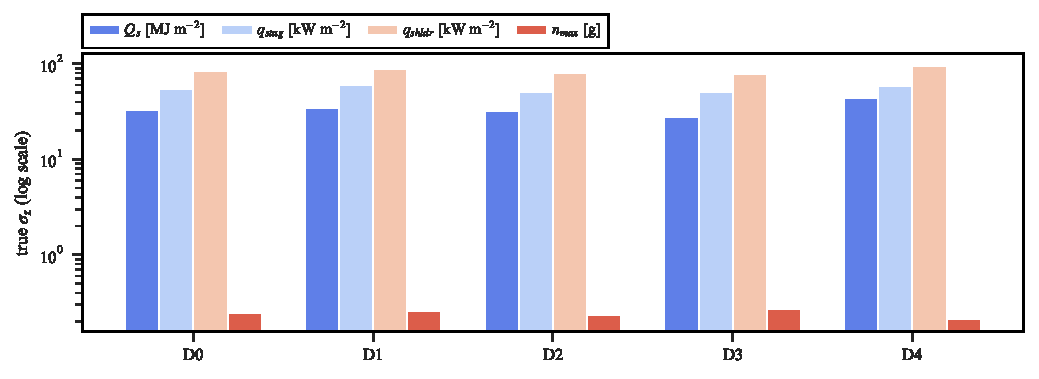
\includegraphics[width=\linewidth]{fig6_probe_true_sigma}
\caption{True uncertainty-driven dispersion $\sigma_z$ of the five probe
  designs ($5\times60$ simulator runs, $t_{\max}=\SI{14400}{\s}$) against
  the final-gate surrogate RMSE. Ratios $\sigma_z/\mathrm{RMSE}=1.6$--$5.6$
  justify the variance-inflated $\sigma_{Q_s}$ objective
  \eqref{eq:infl}.}
\label{fig:probe}
\end{figure}

\begin{figure}[htbp]
\centering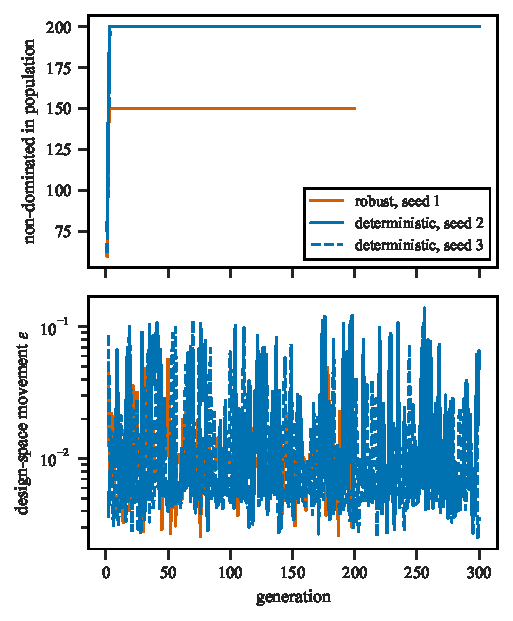
\includegraphics[width=\linewidth]{figS1_nsga2_convergence}
\caption{NSGA-II convergence evidence: per-generation non-dominated count
  and design-space movement ($\varepsilon$) for the robust run and two
  deterministic seeds. Fronts fill by generation 3--4; the movement decays
  to a recombination-noise floor of $6\times10^{-3}$--$10^{-2}$.}
\label{fig:convergence}
\end{figure}

%======================================================================
% 5. RESULTS: DETERMINISTIC VS ROBUST FRONTS
%======================================================================
\section{Results: deterministic vs robust fronts}
\label{sec:results}

The deterministic front was generated on the surrogate at $\mathbf{z}_0$ and
then re-evaluated through the moment engine; the robust front is native to
it. Unless stated otherwise, every number in this section is a
common-random-number moment at $n_z=2000$ with the inflated $\sigma$ of
Eq.~\eqref{eq:infl}. Both final populations are feasible in their own
formulation and, at reporting precision, non-dominated.

\subsection{Front geometry and the dispersion floor}
\label{sec:fronts}

Figure~\ref{fig:front} places both fronts in the
$\mathrm{E}[Q_s]$--$\sigma_{Q_s}$ plane. Two features organize everything
that follows. The first is the dispersion floor: the minimum attainable
$\sigma_{Q_s}$ is \SI{16.4}{\mega\joule\per\square\metre} (coefficient of
variation 19.9\%), and it is the same for both fronts --- a property of
the uncertainty model, principally the $\gamma_0$ dispersion, that no
shape in the studied three-parameter space reaches below. The floor is
geometry-insensitive \emph{within this design space and uncertainty
model}; Section~\ref{sec:sens} shows how it scales when the assumed
dispersions change, and we make no claim of a universal physical bound. The second is where the fronts sit relative
to that floor: the robust front tracks it closely over its whole length,
while the deterministic front, optimized without any dispersion term,
wanders up to three times higher in $\sigma_{Q_s}$ at comparable expected
heat load. The projections of Fig.~\ref{fig:projections} show the same
structure in the performance objectives: the fronts overlap substantially
in $(\eta_V,\mathrm{E}[Q_s])$ and $(\mathrm{E}[sg],\mathrm{E}[Q_s])$, so
robustness is not bought with a separate region of the performance space
but with different designs at like performance.

\begin{figure}[htbp]
\centering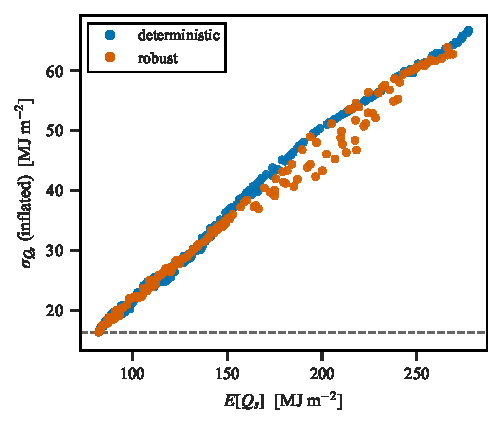
\includegraphics[width=\linewidth]{fig1_front_sigma}
\caption{Deterministic (blue) and robust (vermillion) fronts in the
  $\mathrm{E}[Q_s]$--$\sigma_{Q_s}$ plane (common-random-number moments,
  $n_z=2000$, inflated $\sigma$). Dashed: geometry-insensitive dispersion
  floor $\sigma_{Q_s}=\SI{16.4}{\mega\joule\per\square\metre}$ (CV
  19.9\%), identical on both fronts -- set by the $\gamma_0$ dispersion,
  not by shape.}
\label{fig:front}
\end{figure}
\begin{figure}[htbp]
\centering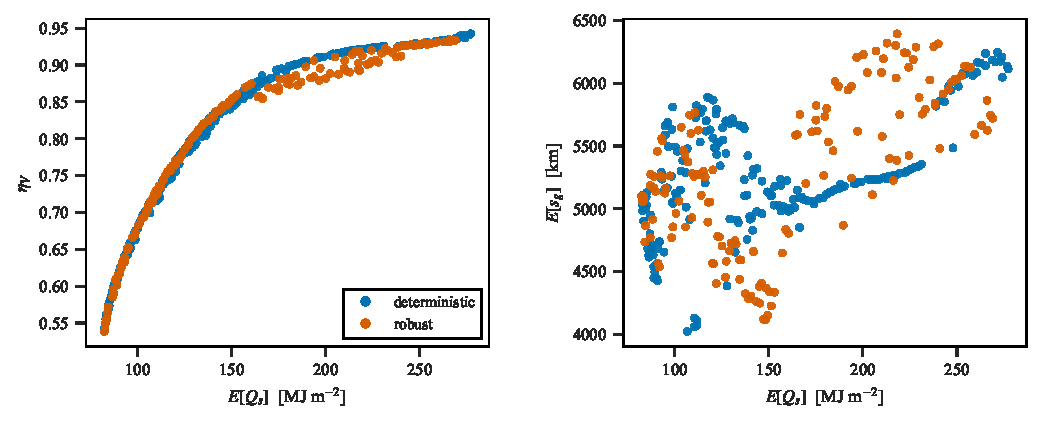
\includegraphics[width=\linewidth]{fig4_front_projections}
\caption{Front projections: volumetric efficiency $\eta_V$ and expected
  range $\mathrm{E}[sg]$ versus $\mathrm{E}[Q_s]$.}
\label{fig:projections}
\end{figure}

\subsection{Matched-performance comparison}
\label{sec:matched}

Front medians are not comparable across a three- against four-objective
formulation, so the comparison is made design against design. A
deterministic design and a robust design form a \emph{matched pair} when
the robust design matches expected heat load and range within a narrow
window ($\mathrm{E}[Q_s]$ at most 2\% higher, $\mathrm{E}[sg]$ at most 2\%
lower); the quantity of interest is then the $\sigma_{Q_s}$ reduction the
robust design achieves at that performance. Of the 200 deterministic
designs, 196 have at least one robust match --- a median of 26 eligible
partners each --- yielding 5{,}371 pairs. In 98.1\% of those pairs the
robust design has the lower $\sigma_{Q_s}$, and the median cut at pair
level is 27.5\% (quartiles 14--47\%; Table~\ref{tab:matched}). These are
descriptive statistics of the constructed comparison set: the 5{,}371
pairs share 196 deterministic and 150 robust designs, so they are not
independent trials, and no sampling interval is attached to them; their
stability across optimizer seeds is reported separately
(Appendix~\ref{app:seeds}).

Because a deterministic design typically has many eligible partners, any
design-level summary depends on the partner-selection rule, and we report
two bounds of it (Table~\ref{tab:matched}, Fig.~\ref{fig:matched}).
Selecting the eligible partner with the lowest $\sigma_{Q_s}$ --- the
envelope of the robust front at matched performance, and the design an
engineer would actually adopt --- improves 99.5\% of the 196 designs,
with a median cut of 35.0\%. This selection examines the outcome, so it
is complemented by a prespecified rule that cannot: the eligible partner
\emph{nearest in relative performance space} (Euclidean distance in the
two matching ratios, ties broken by front index). Under that rule 84.2\%
of designs are still improved, with a median cut of 4.3\%. The gap
between the two rules is structural, not statistical: at matched
performance the robust front offers a spread of $\sigma_{Q_s}$ --- a
median factor 1.49 between the extreme eligible partners --- because
$\sigma_{Q_s}$ is itself an objective traded against $\eta_V$. The
nearest performance neighbour is typically a member of that spread whose
$\sigma_{Q_s}$ resembles the deterministic design's own --- in the
low-load tercile the chosen partners sit at the 11th
$\sigma$-percentile of the robust front (both fronts sit on the floor
there), in the high-load tercile at the 81st (the robust front's own
high-$\sigma$ extreme members) --- while the envelope is the lower edge
of the same spread. Both rules locate the advantage in the same place:
the envelope cut grows monotonically across heat-load terciles of the
deterministic front (14.6\%, 45.8\%, 63.7\%), while the
nearest-neighbour cut peaks in the middle tercile (1.5\%, 14.5\%,
2.2\%). Restricting the window to bind in both legs (both ratios
within $\pm$2\%; 136 of the 5{,}371 pairs) collapses the median cut to
0.4\%: the advantage is carried by the one-sided slack the window
allows --- robust designs delivering less expected heat load at no less
range --- rather than by equal-performance designs differing in
$\sigma_{Q_s}$ alone. The worst members also improve: the maximum exceedance
probabilities over each front roughly halve under the robust formulation
(Table~\ref{tab:matched}, lower rows).

\begin{figure}[htbp]
\centering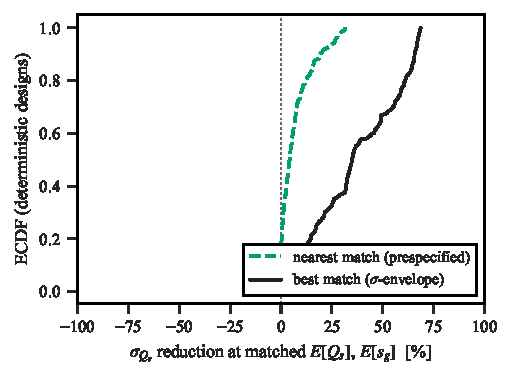
\includegraphics[width=\linewidth]{fig2_matched_sigma_cut}
\caption{ECDF over deterministic designs of the $\sigma_{Q_s}$ reduction
  at matched performance (window $\mathrm{E}[Q_s]+2\%$,
  $\mathrm{E}[sg]-2\%$) under two partner-selection rules: the
  prespecified nearest-performance match (green dashed) and the
  lowest-$\sigma$ eligible partner, i.e.\ the robust front's
  $\sigma$-envelope at matched performance (black). Median cuts 4.3\%
  and 35.0\%; 196/200 designs matched; 98.1\% of the 5{,}371 matched
  pairs favour the robust front.}
\label{fig:matched}
\end{figure}
\begin{table}[htbp]
\centering
\caption{Matched-performance comparison of the fronts (window
  $\mathrm{E}[Q_s]+2\%$, $\mathrm{E}[sg]-2\%$, inflated $\sigma$).}
\label{tab:matched}
\begin{tabular}{lc}
\toprule
statistic & value \\
\midrule
deterministic designs with $\geq$1 robust match & 196 / 200 \\
matched (det, robust) pairs & 5{,}371 \\
pairs with $\sigma_{\mathrm{rob}}<\sigma_{\mathrm{det}}$ & 98.1\% \\
pair-level median $\sigma_{Q_s}$ cut & 27.5\% \\
design-level: designs improved by best match ($\sigma$-envelope) &
  99.5\% \\
design-level median best-match cut (Fig.~\ref{fig:matched}) & 35.0\% \\
design-level: designs improved by nearest match (prespecified) &
  84.2\% \\
design-level median nearest-match cut (Fig.~\ref{fig:matched}) &
  4.3\% \\
median $\sigma$-spread of eligible partners (max/min) & 1.49 \\
worst-member $P(q_{\mathrm{stag}}>\mathrm{lim})$, det / robust &
  6.8\% / 4.8\% \\
worst-member $P(q_{\mathrm{shldr}}>\mathrm{lim})$, det / robust &
  10.0\% / 6.6\% \\
\bottomrule
\end{tabular}
\end{table}

\subsection{The hidden cost of deterministic design}
\label{sec:audit}

The deterministic front satisfies every constraint of Eq.~\eqref{eq:detcon}
at $\mathbf{z}_0$ exactly. Under the uncertainty model, however, a
point-feasible design is a distribution, and the deterministic formulation
never looks at that distribution. The post-hoc audit
(Table~\ref{tab:audit}, Fig.~\ref{fig:violation}) quantifies what is
concealed. The median $\sigma_{Q_s}$ hidden on the deterministic front is
\SI{30.3}{\mega\joule\per\square\metre} (median coefficient of variation
22.8\%). One in four deterministic designs carries a stagnation-heating
exceedance probability above 1\% (maximum 6.8\%), and nearly one in four a
shoulder-heating exceedance probability above 1\% (maximum 10.0\%); the
load-factor constraint is never active under dispersion. Requiring
robust-style feasibility ($\mathrm{E}+2\sigma$) would remove 8\% of the
deterministic front. None of this is visible from the deterministic
problem's own outputs, which report all constraints as satisfied ---
Section~\ref{sec:verification} confirms the largest of these probabilities
against the true simulator.

\begin{figure}[htbp]
\centering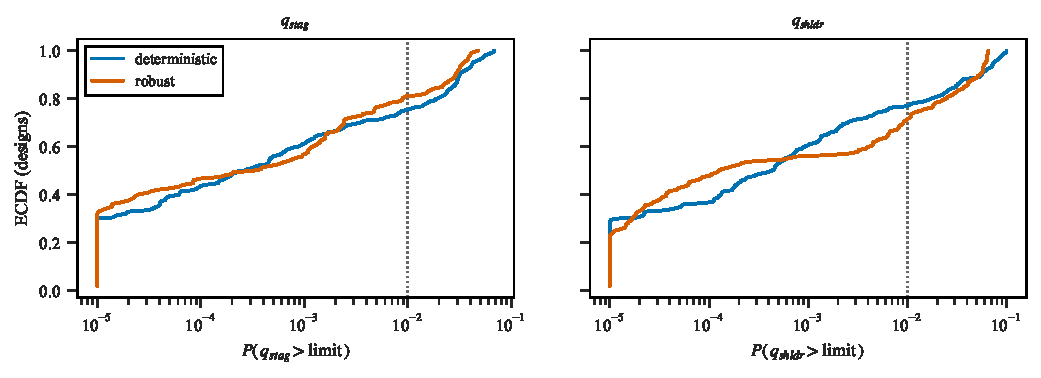
\includegraphics[width=\linewidth]{fig3_violation_ecdf}
\caption{Exceedance probabilities over each front. The deterministic
  front reaches $P(q_{\mathrm{stag}}>\mathrm{lim})=6.8\%$ and
  $P(q_{\mathrm{shldr}}>\mathrm{lim})=10.0\%$ at its worst members; the
  robust front roughly halves both (4.8\% / 6.6\%).}
\label{fig:violation}
\end{figure}
\begin{table}[htbp]
\centering
\caption{Post-hoc fragility audit of the deterministic front (moments
  under the uncertainty model, $n_z=2000$).}
\label{tab:audit}
\begin{tabular}{lc}
\toprule
statistic & value \\
\midrule
$\sigma_{Q_s}$ median (CV median) & \SI{30.3}{\mega\joule\per\square\metre} (22.8\%) \\
$P(q_{\mathrm{stag}}>\mathrm{lim})>1\%$ & 25\% of designs (max 6.8\%) \\
$P(q_{\mathrm{shldr}}>\mathrm{lim})>1\%$ & 23.5\% of designs (max 10.0\%) \\
$P(n_{\max}>\mathrm{lim})>1\%$ & 0\% of designs \\
$P(\mathrm{slow})$ & 0.35--0.49 \\
robust-feasible fraction (E$+2\sigma$) & 92\% \\
\bottomrule
\end{tabular}
\end{table}

\subsection{Knee designs}
\label{sec:knees}

For a concrete comparison, the knee of each front was extracted with the
anchor-hyperplane criterion of Branke et al.\ \cite{branke2004knees}; the
robust front's anchor points are affinely dependent (one design anchors
both $\mathrm{E}[Q_s]$ and $\sigma_{Q_s}$), so a pseudo-weight criterion is
used there as the documented fallback. Table~\ref{tab:knees} lists both
knees, the robust design nearest the deterministic knee in the
$(\mathrm{E}[Q_s],\mathrm{E}[sg])$ plane, and simulator-truth nominal
values for each.

The two knees occupy different points of the trade. The robust knee is the
better vehicle by the nominal simulator as well: volumetric efficiency
0.857 against 0.745 and a nominal range of 11{,}321 against 7{,}465~km,
paid for with a higher nominal heat load (183.9 vs
\SI{128.8}{\mega\joule\per\square\metre}). The matched comparison is more
sobering and more instructive: the robust design closest to the
deterministic knee in expected performance cuts $\sigma_{Q_s}$ by only
3.7\%, because the deterministic knee already sits near the dispersion
floor. The matched-pair advantage of Fig.~\ref{fig:matched} lives
overwhelmingly in the higher-performance region of the front, where heat
load and range are pushed toward their limits and dispersion grows; at the
low-load corner, both formulations converge on the same near-floor designs.
The slow-family probability separates the knees sharply (19\% against 48\%):
the robust knee buys its range partly through lofted, dispersed
trajectories, a trade the deterministic formulation cannot even express.

\begin{table}[htbp]
\centering
\caption{Knee-point designs of each front and the robust design nearest
  the deterministic knee in the $(\mathrm{E}[Q_s],\mathrm{E}[sg])$ plane;
  robust lens ($n_z=2000$), nominal values from the simulator at
  $\mathbf{z}_0$.}
\label{tab:knees}
\begin{tabular}{lccc}
\toprule
quantity & det knee & robust knee & robust matched \\
\midrule
$R_n$ [m]                  & 5.60  & 4.84  & 5.20 \\
$R_s$ [m]                  & 0.020 & 0.022 & 0.021 \\
$\theta_c$ [deg]           & 37.0  & 21.6  & 40.9 \\
$\eta_V$ [-]               & 0.745 & 0.857 & 0.725 \\
$Q_s$ at $\mathbf{z}_0$ (sim) [\si{\mega\joule\per\square\metre}]
                           & 128.8 & 183.9 & 119.8 \\
$sg$ at $\mathbf{z}_0$ (sim) [km]
                           & 7{,}465 & 11{,}321 & 6{,}514 \\
$\mathrm{E}[Q_s]$ [\si{\mega\joule\per\square\metre}]
                           & 117.4 & 164.1 & 110.6 \\
$\sigma_{Q_s}$ [\si{\mega\joule\per\square\metre}]
                           & 24.8  & 37.3  & 23.9 \\
$\mathrm{E}[sg]$ [km]      & 5{,}887 & 5{,}586 & 5{,}766 \\
$P(q_{\mathrm{shldr}}>\mathrm{lim})$ [\%]
                           & 0.01  & 0.32  & 0.004 \\
$P(\mathrm{slow})$ [\%]    & 19.4  & 48.0  & 43.3 \\
\bottomrule
\end{tabular}
\end{table}

\begin{figure}[htbp]
\centering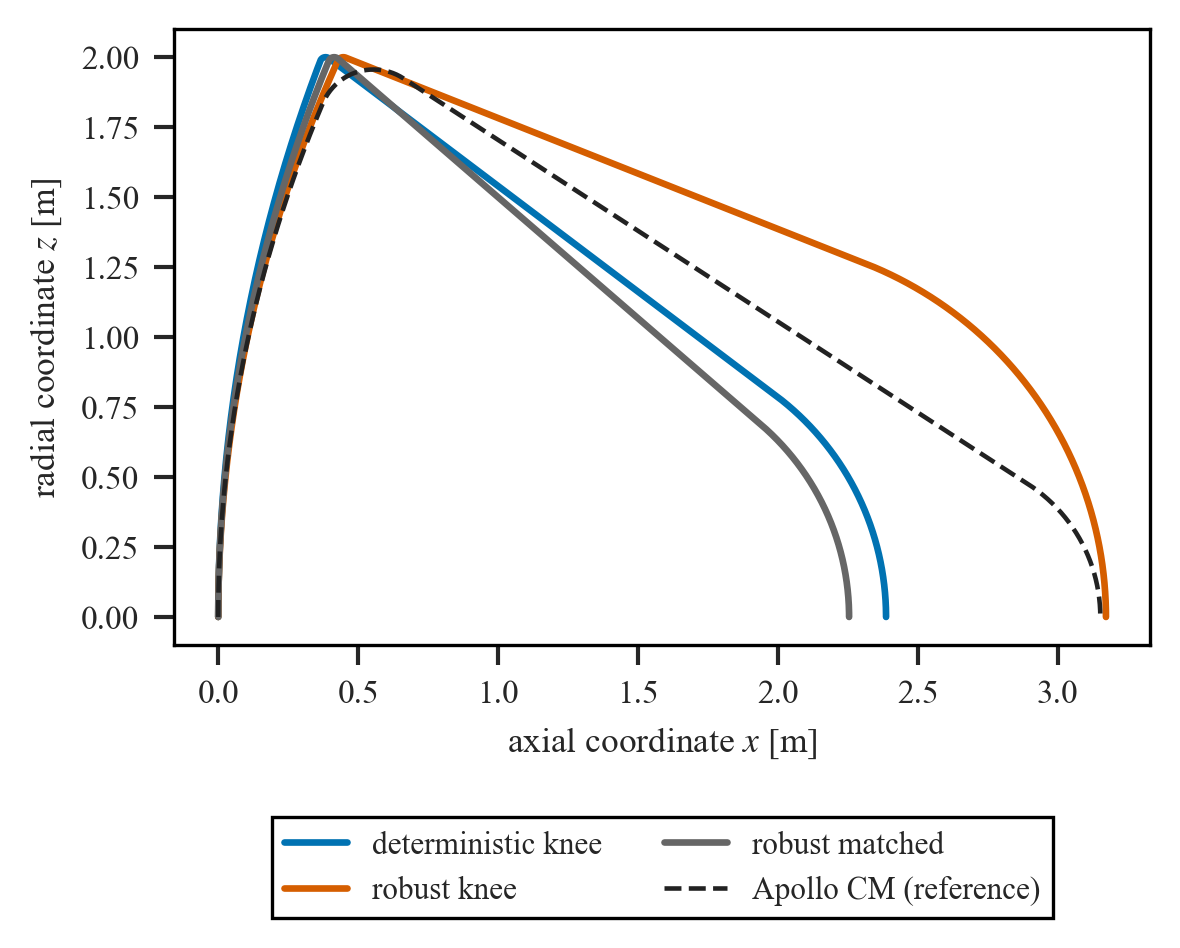
\includegraphics[width=0.8\linewidth]{fig7_silhouettes_knees}
\caption{Meridional outlines of the knee designs and the robust matched
  design of Table~\ref{tab:knees}, with the Apollo command module
  (dashed; drawn at its own body radius of \SI{1.956}{\metre}) for scale.
  The robust knee is the blunter, lower-cone shape
  ($R_n=\SI{4.84}{\metre}$, $\theta_c=21.6^\circ$); the deterministic
  knee and the matched design sit close together
  ($R_n\approx\SI{5.2}{\metre}$--$5.6$, $\theta_c=37$--$41^\circ$).}
\label{fig:silhouettes}
\end{figure}

\subsection{Design-space view}
\label{sec:designspace}

Figure~\ref{fig:designspace} maps the inflated $\sigma_{Q_s}$ over the
design space (300-point scan, $r_s$ slice) with both fronts overlaid. Both
formulations settle in the low-dispersion region of the space --- the
deterministic one by constructive accident, since low heat load and low
dispersion correlate through the same shallow-entry physics --- and the
floor binds everywhere on the map's cold side. The same scan confirms the
$P(\mathrm{slow})$ finding of Section~\ref{sec:robform}: family
probability varies only between 0.34 and 0.59 across the entire space.
Geometry does not buy direct descent under a $\pm0.5^\circ$
flight-path-angle dispersion; corridor and guidance levers would have to.

\begin{figure}[htbp]
\centering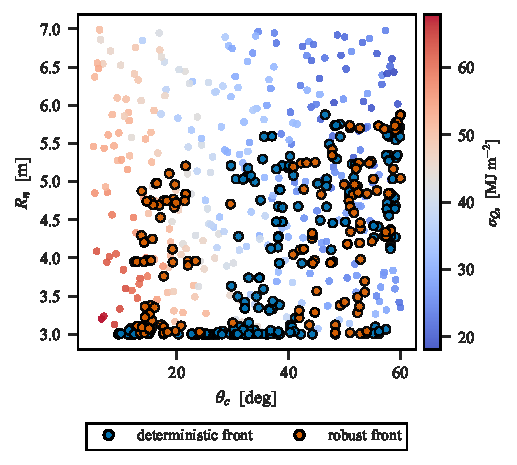
\includegraphics[width=\linewidth]{fig5_design_space_sigma_map}
\caption{Inflated $\sigma_{Q_s}$ over the design space (300-point scan,
  $r_s$ slice) with both fronts. Both fronts hug the low-dispersion
  region; the floor binds everywhere.}
\label{fig:designspace}
\end{figure}

\subsection{Deterministic exploitation of surrogate epistemics}
\label{sec:exploit}

The audit surfaced one more consequence of point-prediction optimization,
this one methodological. Fifty-four of the 200 deterministic designs carry
a surrogate range prediction at $\mathbf{z}_0$ above
\SI{20015}{\kilo\metre} --- above the antipodal great-circle distance, the
physical maximum of the quantity being optimized. The mechanism is the
slow-family range GP: in the deterministic problem, $sg(\mathbf{z}_0)$ is a
plain mixture prediction, and in the lofted corner the slow-GP mean
extrapolates far outside its training support (at the deterministic knee
the slow-GP mean is $10^5$~km). The optimizer, maximizing range, walked
straight into that blind spot: the surrogate claims
$\SI{26004}{\kilo\metre}$ at the deterministic knee where the simulator
returns \SI{7465}{\kilo\metre} --- a factor of 3.5. The robust formulation
does not fall into the same trap, for a structural reason:
$\mathrm{E}[sg]$ is formed by averaging the mixture over the uncertainty
sample, which damps any single extrapolating component, and the resulting
robust front spans $\mathrm{E}[sg]=4{,}117$--$6{,}393$~km, entirely within
the physical envelope. The lesson generalizes: a probabilistic surrogate
optimized through its point predictions will be exploited wherever its
mean leaves the data, and moment objectives --- or any formulation that
averages over the uncertainty space --- self-regulate against exactly this
failure. All nominal-range values quoted in this paper for specific
designs (Table~\ref{tab:knees} and Section~\ref{sec:verification}) come
from the simulator, never from the surrogate at $\mathbf{z}_0$.

\subsection{Sensitivity of the comparison to the uncertainty model and
matching construction}
\label{sec:sens}

The comparison rests on one uncertainty model and one matching window, so
both were stress-tested. Each front was re-evaluated through the same
common-random-number moment engine under five alternative uncertainty
models --- the aerodynamic band widened and narrowed
($\sigma_k=0.03,\,0.07$), the two scale factors correlated
($\rho=0.8$, addressing the weakest assumption of
Section~\ref{sec:uncertainty}), and the flight-path-angle dispersion
halved and enlarged by half ($\sigma_{\gamma_0}=0.25^\circ,\,0.75^\circ$)
--- using the same Latin-hypercube seed, with shared $\gamma_0$/$V_0$
quantiles wherever the distributions allow. The baseline configuration
reproduces the statistics of Tables~\ref{tab:matched} and \ref{tab:audit}
exactly, anchoring the comparison. Table~\ref{tab:sens} reports the
resulting statistics.

\begin{table}[htbp]
\centering
\caption{Sensitivity of the comparison statistics to the uncertainty
  model (both fronts re-evaluated through the same moment engine,
  $n_z=2000$; baseline column reproduces Tables~\ref{tab:matched} and
  \ref{tab:audit}).}
\label{tab:sens}
\begin{tabular}{lcccccc}
\toprule
statistic & base & $\sigma_k{=}0.03$ & $\sigma_k{=}0.07$ &
$\rho{=}0.8$ & $\sigma_{\gamma_0}{=}0.25^\circ$ &
$\sigma_{\gamma_0}{=}0.75^\circ$ \\
\midrule
$\sigma_{Q_s}$ floor, robust front [MJ/m$^2$]
  & 16.4 & 16.0 & 16.8 & 16.2 & 13.0 & 20.5 \\
det.-front $\sigma_{Q_s}$ median [MJ/m$^2$]
  & 30.3 & 29.9 & 30.8 & 30.1 & 24.1 & 37.4 \\
det.-front max $P(q_{\mathrm{shldr}}>\mathrm{lim})$ [\%]
  & 10.0 & 10.0 & 9.9 & 9.9 & 1.5 & 17.8 \\
det.\ designs with a match
  & 196 & 195 & 197 & 195 & 195 & 188 \\
matched pairs
  & 5{,}371 & 5{,}316 & 5{,}418 & 5{,}238 & 7{,}398 & 3{,}719 \\
pairs favouring robust [\%]
  & 98.1 & 98.1 & 98.0 & 98.0 & 98.6 & 96.3 \\
pair-level median $\sigma$ cut [\%]
  & 27.5 & 27.6 & 27.2 & 27.0 & 36.6 & 17.2 \\
design-level median $\sigma$ cut [\%]
  & 35.0 & 35.4 & 34.4 & 35.2 & 43.0 & 33.8 \\
\bottomrule
\end{tabular}
\end{table}

Three observations. First, the comparison is indifferent to the
aerodynamic model-form specification: across $\pm40\%$ of the scale band
and a strongly correlated pair, every statistic moves within a percentage
point, and the dispersion floor stays between 16.0 and
\SI{16.8}{\mega\joule\per\square\metre}. The floor is not an artefact of
the aerodynamic uncertainty --- which is exactly what
Section~\ref{sec:fronts} claims. Second, the entry-state dispersion moves
the absolute levels as it must (the floor scales with
$\sigma_{\gamma_0}$: 13.0, 16.4, \SI{20.5}{\mega\joule\per\square\metre}
at 0.25, 0.5, 0.75$^\circ$; the hidden worst-case exceedance probability
scales from 1.5\% to 17.8\%; robust-style feasibility of the deterministic
front from 100\% down to 78.5\%), but the comparison conclusions do not:
across a factor-three range of $\sigma_{\gamma_0}$, the fraction of pairs
favouring the robust front stays between 96.3 and 98.6\%, and the
design-level median cut between 33.8 and 43.0\%. The fragility finding is
a faithful image of the dispersion it reflects, not of one chosen band.
Third, the matching construction is not doing the work: with the window
widened from $\pm1\%$ to $\pm5\%$, the pair count grows from 4{,}766 to
7{,}136 while the fraction favouring robust moves only from 99.1\% to
94.4\%, the pair-level median cut stays within $27.5\pm1$ percentage
points, and the design-level median cut within $35.9\pm1.5$. A further
variation addresses the range leg specifically, because that leg carries
the surrogate's $\mathrm{E}[sg]$ bias (Section~\ref{sec:verification}):
holding the heat-load leg at $+2\%$ and widening only the range leg ---
to 5, 10, 15\%, and complete removal --- moves the pair preference from
98.1\% to no less than 97.2\% and the pair-level median cut from 27.5\%
to 32.2\%, the cuts growing because lower-range robust designs disperse
less. No differential bias of the surrogate's range prediction can
therefore overturn the comparison through the matching construction.
Finally, the
headline statistics are stable across optimizer seeds: three independent
robust runs give matched-pair preferences of 97.4--98.1\%, design-level
median cuts of 31.9--35.0\%, and the same dispersion floor to three
significant figures (16.36--\SI{16.4}{\mega\joule\per\square\metre};
Appendix~\ref{app:seeds}); the nearest-match statistic is the most
seed-sensitive (designs improved 68.9--84.2\%) but its conclusion holds
on every seed.

%======================================================================
% 6. VERIFICATION AGAINST THE TRUE SIMULATOR
%======================================================================
\section{Verification against the true simulator}
\label{sec:verification}

Every result so far rests on the surrogate moment engine, so five designs
were re-examined against the trajectory simulator itself: the deterministic
and robust knees, the robust matched design of Table~\ref{tab:knees}, the
most fragile deterministic design (the front's worst shoulder-heating
exceedance probability --- the audit headline), and the minimum-dispersion
robust design (the floor claim). Each was propagated with $N=300$
uncertainty samples drawn from the frozen distributions
($t_{\max}=\SI{14400}{\s}$), 1{,}500 simulator runs in total, about 23~s
each. There were no integration failures and 1{,}499 of 1{,}500 runs
captured.

Table~\ref{tab:verify} summarizes the comparison for the three designs that
stress the claims. Expected heat load is verified to within $-3.2$ to
$+1.4\%$ across all five designs, and $\sigma_{Q_s}$ to within a few
percent (MC slightly lower throughout); in particular the floor survives:
the minimum-dispersion design measures $\sigma_{Q_s}=
\SI{15.4}{\mega\joule\per\square\metre}$ in simulation against the claimed
\SI{16.4}{\mega\joule\per\square\metre} --- the floor is real, and the
inflated-$\sigma$ construction errs on the conservative side. The
peak-heating $\mathrm{E}+2\sigma$ constraints are met with 1--3\%
margin. The audit's headline number is confirmed at its worst point: the
fragile deterministic design shows $P(q_{\mathrm{shldr}}>\text{limit})=
29/299=9.7\%$ in simulation against the surrogate's promised 10.0\%, and
$P(q_{\mathrm{stag}}>\text{limit})=7.4\%$ against 6.8\%. The 299
denominators are exact bookkeeping rather than a quiet exclusion: the
fragile design's shallowest draw ($\gamma_0=-0.52^\circ$, three standard
deviations above nominal, with $k_{CL}=1.07$) lofts into a long skip
trajectory that is still airborne at the integration horizon
$t_{\max}=\SI{14400}{\s}$ --- a physical escape of the terminal event
rather than an integration failure, and non-capturing under both
guidance laws. Its recorded heat load and shoulder heating at cutoff lie
far below the limits; counting that run as an exceedance or as a
non-exceedance brackets the estimate between 29/300 and 30/300
(9.7--10.0\%), so the verification statement is insensitive to its
treatment. (Under the alternate law of Section~\ref{sec:guidance} the
same brackets are 17.0--17.3\% around the reported 17.1\%.) Both knees
show zero exceedances in 300 runs, which bounds their true exceedance
probabilities below $\approx$1\% (rule of three). Slow-family
probabilities agree within about six percentage points.

\begin{table}[htbp]
\centering
\caption{Monte-Carlo verification of the surrogate moment engine
  ($N=300$ true-simulator runs per design). Diff. = (MC $-$ surrogate)
  in \% of the surrogate value.}
\label{tab:verify}
\begin{tabular}{lccc}
\toprule
quantity & det knee & robust knee & det fragile \\
\midrule
$\mathrm{E}[Q_s]$ diff.        & $+0.1\%$  & $+1.4\%$  & $-3.2\%$ \\
$\sigma_{Q_s}$ MC / predicted  & 23.9/24.8 & 36.2/37.3 & 65.9/66.7 \\
$\mathrm{E}[sg]$ diff.         & $-24.6\%$ & $-8.8\%$  & $-20.1\%$ \\
$P(\mathrm{slow})$ MC / pred.  & 0.40/0.45 & 0.46/0.48 & 0.49/0.49 \\
$P(q_{\mathrm{stag}})$ MC / pred. & 0/300 / $<0.1\%$ & 0/300 & 7.4\%/6.8\% \\
$P(q_{\mathrm{shldr}})$ MC / pred. & 0/300 / $<0.1\%$ & 0/300 & \textbf{9.7\%/10.0\%} \\
\bottomrule
\end{tabular}
\end{table}

One systematic discrepancy survives verification and is disclosed rather
than tuned away: predicted $\mathrm{E}[sg]$ is high by 8.8--28.1\% on all
five designs (standard errors 2.7--10.1\%). The bias has a single,
identifiable cause. The mixture prediction averages a lognormal for each
family, and the mean of a lognormal amplifies the fitted variance; for the
slow family, whose fitted log-standard-deviation is large by necessity
(Section~\ref{sec:gp}), that amplification is severe --- the same mechanism
that produced the 3.5$\times$ nominal-range extrapolation of
Section~\ref{sec:exploit}, here in its mild, moment-level form. Monte-Carlo
truth for the five designs puts $\mathrm{E}[sg]$ at 4.1--5.1~Mm. What
this bias does to the matched-pair comparison is a fair question, and
the answer is not that it cancels: the window holds $\mathrm{E}[sg]$
equal only in surrogate units, so what matters is the
\emph{differential} bias between matched designs. The measured bias is
design-specific --- multiplicative factors 1.10--1.39 across the five
verified designs, with no systematic difference between the fronts
(deterministic 1.25--1.33, robust 1.10--1.39) --- and at the
matched knee pair verified end to end (deterministic knee against the
robust design of Table~\ref{tab:knees}) it moves the range
ratio from $-2.1\%$ in surrogate units to $-6.6\%$ in simulation, while
the comparison itself survives: the heat-load leg of the window holds
with margin ($-6.4\%$), and the $\sigma_{Q_s}$ cut grows from 3.7\% to
5.1\%.

The differential bias can also be measured directly, at the pairs where
it had the best chance to distort the comparison. The five most
adversarial matched pairs were re-verified end to end against the
simulator: one pair per expected-heat-load quintile, each deterministic
member chosen with a predicted $\sigma_{Q_s}$ cut at least the
pair-level median of 27.5\% and the least range slack in its window ---
precisely where a surrogate error could most plausibly manufacture or
break a match. Both members of every pair were propagated with the same
$N=300$ shared uncertainty samples (3{,}000 further simulator runs;
2{,}999 captured, the single non-capture being one shallow lofted draw
of the fifth pair's deterministic member, of the kind already described
above). The comparison survives intact. The predicted $\sigma_{Q_s}$
cuts of $+30.9$ to $+67.1\%$ measure $+32.0$ to $+68.5\%$ in simulation
--- per-pair agreement within 1.5 percentage points, and the true cut
the larger in four of five pairs. The heat-load leg of the window is
likewise confirmed: member ratios of expected heat load $0.42$--$0.74$
predicted against $0.40$--$0.74$ measured, the largest deviation
(pair~4: 0.402 against 0.420) understating the robust advantage. The
range ratios move from the matched $-2.0\%$ in surrogate units to
$-5.2$ to $+8.1\%$ measured (standard errors near $\pm 5\%$): the
differential bias is real but bounded, and at these five pairs it runs
in the robust front's favour --- the robust members' measured
$\mathrm{E}[sg]$ inflation is smaller on average (1.23 against 1.26;
factors 1.14--1.37 deterministic against 1.10--1.33 robust, all inside
the envelope above) --- so the mean measured range ratio is 1.01:
matched robust designs give up no range in truth. The matched-pair statistics
of Section~\ref{sec:matched} therefore rest on direct measurement, not
only on the bounds below.

Two bounds cover the pairs not verified directly. First, widening or
removing the range leg of the window leaves the pair statistics intact
(Section~\ref{sec:sens}: preference 97.2--98.1\%, median cut
27.5--32.2\%), so no differential bias of plausible magnitude can
overturn the comparison through the matching. Second, the Monte-Carlo
standard error on $\mathrm{E}[sg]$ at $N=300$ is itself 3.5--4\%, so a
2\% range window is beyond the resolution of any verification budget
this study could afford; the heat-load leg, verified to $-3.2$ to
$+1.4\%$, is what carries the matching. Absolute range values quoted
from the surrogate should be read as conservative-high by 9--37\%
across the fifteen verified designs.

\subsection{Guidance-law sensitivity}
\label{sec:guidance}

The guidance realization was the dominant residual in the end-to-end
validation (Appendix~\ref{app:variants}), so the verification was repeated
under the alternate bank law of Table~\ref{tab:variants} --- Eq.~2.40 as
printed with the 82$^\circ$ command cap, the variant that reproduces the
reference track length to $-1.1\%$ --- re-running the same five designs at
the same 300 uncertainty samples (1{,}500 further simulator runs). The
shifts are systematic rather than erratic: expected heat load moves $-1$
to $-7\%$, expected range $-5$ to $-13\%$, and heat-load dispersion
\emph{increases} by 7--24\% under the more aggressive modulation. Two
results matter. The verified knees remain safe under both laws (zero
exceedances in 300 runs at the deterministic knee and the matched design;
2/300 shoulder exceedances at the robust knee). And the hidden fragility
of the deterministic front survives and amplifies: at the fragile design,
shoulder-heating exceedances rise from 29/299 (9.7\%) to 51/299 (17.1\%)
and stagnation-heating exceedances from 22/299 to 42/299. The concealed
risk is thus not an artefact of one guidance realization --- if anything,
the alternate law is harsher on the point-feasible design. Absolute
dispersion levels, including the floor's magnitude (15.4 to
\SI{19.1}{\mega\joule\per\square\metre} at the floor design), are
guidance-dependent exactly as the claims accounting of
Section~\ref{sec:validation} anticipated; the comparison conclusions, and
the floor's geometry-independence, are not.

%======================================================================
% 7. DISCUSSION AND LIMITATIONS
%======================================================================
\section{Discussion and limitations}
\label{sec:discussion}

\subsection{What the comparison means for design practice}
\label{sec:practice}

Three findings carry weight beyond this specific capsule.

First, the size of the robustness dividend depends on where on the front
one stands. Near the dispersion floor --- the low-heat-load corner ---
deterministic and robust optimization return essentially the same designs,
and a matched comparison there shows cuts of a few percent. The 35\%
design-level median cut --- the robust front's $\sigma$-envelope at
matched performance --- and the near-universal pair-level preference
come from the high-performance region, where constraints are pushed and
dispersion grows quickly; the strict prespecified matching of
Section~\ref{sec:matched} (median cut 4.3\%) is the complementary
reminder that the two fronts also interleave, and that the dividend is
an attainable envelope, not a uniform displacement. A programme
optimized at a comfortable margin
point has less to gain from robust reformulation than one operating near
its limits; the deterministic knee of this study is the cautionary
example, sitting within 3.7\% of the floor while the front behind it hides
10\% exceedance probabilities.

Second, the dispersion floor itself is the sharper design insight. At
$\sigma_{\gamma_0}=0.5^\circ$, no shape in a three-variable capsule space
reduces heat-load dispersion below about \SI{16}{\mega\joule\per\square\metre}
(CV $\approx$ 20\%), the slow-family probability cannot be engineered
below $\approx$0.34, and both fronts bottom out at the same value. The
levers that would move those numbers are not geometric: entry-corridor
targeting, guidance, and, on the modelling side, the aerodynamic
model-form error. When a robust optimization reports an irreducible floor,
the correct reading is not ``robust optimization failed to help'' but
``shape is no longer the active constraint on dispersion'' --- a
conclusion the deterministic formulation cannot produce at all, because it
never sees the dispersion.

Third, the exploitation episode of Section~\ref{sec:exploit} is a warning
for the now-common practice of optimizing probabilistic surrogates through
point predictions. The deterministic optimizer maximized range into a
region where the surrogate mean exceeded the antipodal distance --- the
physical maximum of its own objective --- and nothing in the deterministic
formulation flagged it. Formulations that average over an uncertainty
space are self-limiting against this failure; formulations that do not
should at least carry a prediction-variance or trust-region guard.

\subsection{Limitations}
\label{sec:limitations}

\begin{itemize}
  \item \textbf{Range surrogate.} The slow-family range response is
        irreducible at practical sampling density ($\sim$15\% error), and
        $\mathrm{E}[sg]$ is biased $+9$ to $+28\%$ by lognormal-mean
        inflation (measured, disclosed; Monte-Carlo-true values reported
        for all verified designs). The bias is design-specific (factors
        1.10--1.39 across the verified designs), so the range leg of the
        matching window is a surrogate-space construct rather than a
        cancelled error; it is bounded instead --- the matched statistics
        are insensitive to widening or removing that leg
        (Section~\ref{sec:sens}), the heat-load leg is
        simulator-verified, and the one end-to-end verified pair retains
        its $\sigma_{Q_s}$ advantage in simulation
        (Section~\ref{sec:verification}). Absolute range claims
        rest on simulation, not on the surrogate.
  \item \textbf{Single nominal mission.} The study operates at one entry
        state ($V_0=7.83$~km/s, $\gamma_0=-2^\circ$ nominal): the
        uncertainty model disperses around that point, but other entry
        classes (low-Earth-orbit return, Mars entry) lie outside the
        evidence base. The dispersion floor would scale with the assumed
        dispersions (Section~\ref{sec:sens}); its geometry-independence,
        by contrast, is a structural finding we expect to carry over.
  \item \textbf{Trajectory model.} Three degrees of freedom, planar-point
        mass with the fixed no-skip bank law, no six-degree-of-freedom
        coupling of attitude and entry loads; the guidance realization is
        bracketed by the alternate-law verification of
        Section~\ref{sec:guidance}. Load factors are the
        drag-based metric with the 4--5\% total-force correction noted in
        Section~\ref{sec:traj}.
  \item \textbf{Uncertainty model.} No atmospheric-density dispersion;
        $k_{CD}$ covers model-form drag error only. Entry-state
        dispersions are Gaussian and independent; the aerodynamic scales
        were sized from wind-tunnel residuals at two Mach numbers. The
        5\% band is an engineering assumption informed by that evidence,
        not a fitted posterior
        (Section~\ref{sec:uncertainty}).
  \item \textbf{Front repeatability.} Both formulations were run with
        three optimizer seeds: objective statistics coincide, robust
        cross-seed domination is 3--10\% (tighter than the deterministic
        formulation's $\le$14\%), and the headline matched statistics
        reproduce within a few percentage points
        (Appendix~\ref{app:seeds}). Residual seed sensitivity at the
        front margins is not fully excluded.
  \item \textbf{Vehicle model.} Fixed Apollo-density mass model and no
        thermal-protection or structural coupling; $Q_s$ serves as a
        proxy for thermal-protection-system mass rather than a sizing
        calculation.
\end{itemize}

The natural continuations are a reliability-based formulation with explicit
probabilistic constraints (for which the verified exceedance statistics
here provide calibration points), atmospheric-density uncertainty, and a
six-degree-of-freedom extension of the trajectory layer. The comparison
machinery --- one validated physics core, a common-random-number moment
engine, matched-pair statistics, and simulator-level verification --- is
formulation-agnostic and carries over unchanged.

%======================================================================
% 8. CONCLUSIONS
%======================================================================
\section{Conclusions}
\label{sec:conclusions}

Deterministic and robust formulations of a three-objective capsule shape
optimization --- maximize volumetric efficiency, minimize integrated heat
load, maximize range --- were solved on one validated aerothermal model and
one set of Gaussian-process surrogates, with an uncertainty model combining
entry-state dispersion ($\gamma_0$, $V_0$) and aerodynamic model-form scales
($k_{CD}$, $k_{CL}$) sized from wind-tunnel validation residuals. A
common-random-number moment engine made the two fronts directly comparable,
and 1{,}500 simulator runs verified the findings against the true model.

At matched expected performance, robust designs reduced heat-load
dispersion in 98.1\% of 5{,}371 matched design pairs, with a median cut
of 27.5\% at pair level and 35.0\% against the robust front's
$\sigma$-envelope at matched performance (4.3\% under the strictest
prespecified matching rule); these statistics are insensitive to
$\pm40\%$ perturbation of the aerodynamic uncertainty band, to
correlation between the aerodynamic scale factors, and to the matching
window --- including removal of its range leg, which carries the
surrogate's measured range bias --- and remain
qualitatively unchanged across a factor-three range of flight-path-angle
dispersion. The deterministic front, feasible at every point at
nominal conditions, concealed shoulder-heating exceedance probabilities up
to 10.0\%, confirmed at 9.7\% by Monte-Carlo simulation at its most
fragile design --- rising to 17.1\% under an alternate guidance
realization --- and roughly one in four of its designs exceeded a 1\%
exceedance probability on stagnation or shoulder heating. A
geometry-insensitive dispersion floor of
\SI{16}{\mega\joule\per\square\metre} (CV $\approx$ 20\%) bounded both
fronts identically within the studied design space and uncertainty model:
under the assumed flight-path-angle dispersion, shape is not an active
lever on heat-load spread, and reducing it further requires corridor,
guidance, or modelling levers outside the design space. Two methodological results complete the
picture. Optimizing a probabilistic surrogate through point predictions
drove the deterministic front into a slow-family extrapolation region
where predicted range exceeded the antipodal distance (a factor of 3.5 at
the knee), while the moment-based formulation self-regulated; and the
mixture surrogate's expected range is biased $+9$ to $+28\%$ by
lognormal-mean inflation, disclosed and bounded here by simulation.

The comparison protocol --- same physics, common random numbers,
matched-pair statistics, post-hoc fragility audit, simulator-level
verification --- is reusable wherever deterministic practice is to be
audited against robust alternatives, and the verified exceedance
statistics provide calibration points for the reliability-based
formulation that follows as future work.


% Flush all pending floats so References is followed only by appendices.
\clearpage

%======================================================================
% REFERENCES (elsarticle-num style)
%======================================================================
\bibliographystyle{elsarticle-num}
\bibliography{refs}

%% Appendices AFTER the references (user preference; matches Elsevier
%% final-article layout).
%======================================================================
% APPENDIX A. REFERENCE-CASE FORENSICS AND MODEL DEVIATIONS
%    (source: capsule_opt/validation/DEVIATIONS.md + RESULTS.md)
%======================================================================
\appendix
\section{Reference-case forensics and model deviations}
\label{app:validation}

This appendix documents, in audit form, the end-to-end comparison against
the Apollo reference case of \cite{dirkx2017entry} summarized in
Section~\ref{sec:validation}: the identified internal inconsistencies of
the reference data, the sensitivity of the comparison to the guidance-law
realization, and the deviations between the present implementation and the
reference method. The purpose is to attribute the residual end-to-end
discrepancies rather than to explain them away.

\subsection{Internal inconsistency of the reference load-factor panel}
\label{app:identity}

For a point-mass entry, the peak load factor and the stagnation heat-rate
curve of one simulation are algebraically coupled, independent of the
trajectory or guidance model:
\begin{equation}
n \;=\; \frac{\dot{q}^{\,2}\,R_{\mathrm{eff}}\,C_D\,A}
            {2\,m\,g\,k^2\,V^4},
\label{eq:identity}
\end{equation}
with $V$ fixed by Mach. This identity holds to $\sim$2\% on our own
trajectories. Applied to the digitized curves of the reference Fig.~7.17(c),
it is violated systematically (Table~\ref{tab:identity}): the ratio between
the printed $n$ panel and the $n$ implied by the printed $\dot{q}$ curve
swings between 0.17 and 0.65, and no single parameter (mass,
$R_{\mathrm{eff}}$, $C_D$, heating constant) reconciles them --- the
rescaling required varies by a factor of two across the Mach range, the
signature of curves from different runs plotted together. The reference's
own $\dot{q}$ curve implies $n_{\max}\approx\SI{11}{g}$ where the panel
prints \SI{4.35}{g}. In addition, the reference table's integrated heat
load (\SI{53.06}{\mega\joule\per\square\metre}) lies below every member of
the variant family of Table~\ref{tab:variants} even though the digitized
$\dot{q}$ curve runs 1.5--2.7$\times$ above ours below $M\approx13$: the
table and the figure disagree with each other, not merely with us. The
load-factor panel is therefore treated as qualitative only, and
peak-load-factor is excluded as a validation target. Apollo flight data
peak at $\sim$3~g (LEO class) to $\sim$7~g (lunar return)
\cite{hillje1969apollo,moseley1969wind}; for the shallower reference case
the 5--7~g class is expected, consistent with the present result
($n_D=5.06$, $n_{\mathrm{tot}}=5.33$~g).

\begin{table}[htbp]
\centering
\caption{Identity check on the digitized reference Fig.~7.17(c): the
  printed load-factor panel versus the load factor implied by the printed
  heat-rate curve through Eq.~\eqref{eq:identity}. A ratio near unity is
  required for self-consistency.}
\label{tab:identity}
\begin{tabular}{rcccc}
\toprule
$M$ & $n$ panel [g] & $\dot{q}$ panel [\si{\kilo\watt\per\square\metre}] &
$n$ implied [g] & ratio \\
\midrule
6.5   & 3.16 & 131 & 19.1 & 0.17 \\
9.4   & 4.05 & 233 & 13.2 & 0.31 \\
12.3  & 4.35 & 371 & 11.0 & 0.40 \\
15.6  & 4.00 & 526 & 8.2  & 0.49 \\
17.5  & 3.50 & 588 & 6.6  & 0.53 \\
19.6  & 2.78 & 616 & 4.9  & 0.57 \\
22.6  & 1.45 & 527 & 2.2  & 0.65 \\
\bottomrule
\end{tabular}
\end{table}

\subsection{Guidance-law sensitivity of the end-to-end comparison}
\label{app:variants}

The reference specifies a no-skip bank law (their Eq.~2.41) but leaves its
realization --- activation gate, saturation, rate limits --- partly open.
Table~\ref{tab:variants} spans a family of realizations. Range and peak
heat rate move in opposite directions across the family: the baseline
reproduces peak heat rate to 0.7\%, the Eq.~2.40-as-printed variant
reproduces track length to $-1.1\%$, and no member reproduces the
reference table and the figure panels simultaneously. The family floor for
integrated heat load is $+16\%$ relative to the table value. The
discrepancies quoted in Section~\ref{sec:validation} ($+32\%$ heat load,
$+16\%$ track length for the baseline) are thus bounded and attributed,
not unexplained.

\begin{table}[htbp]
\centering
\caption{Guidance-variant family on the reference Apollo case (reference
  table values: $Q_s=\SI{53.06}{\mega\joule\per\square\metre}$,
  $sg=\SI{1430.2}{\kilo\metre}$,
  $\dot{q}_{\max}=\SI{0.616}{\mega\watt\per\square\metre}$).}
\label{tab:variants}
\begin{tabular}{lccccc}
\toprule
variant & $Q_s$ & $sg$ & $\dot{q}_{\max}$ & $n_{\mathrm{tot}}$ &
bank onset \\
\midrule
baseline (Eq.~2.41, sin-$\chi$)      & 70.1 ($+32\%$) & 1657 ($+16\%$) &
  \textbf{0.621 ($+0.7\%$)} & 5.33 & $M\,24.4$ \\
gate $\varepsilon{=}0.15$, cap $82^\circ$ & 65.7 ($+24\%$) & 1519 ($+6\%$) &
  0.663 & 6.91 & $M\,25.8$ \\
gate $\varepsilon{=}0.30$, cap $82^\circ$ & 64.2 ($+21\%$) & 1477 ($+3\%$) &
  0.683 & 7.52 & $M\,26.6$ \\
Eq.~2.40 as printed (sin-$\gamma$), cap $82^\circ$ & 61.6 ($+16\%$) &
  \textbf{1414 ($-1\%$)} & 0.722 ($+17\%$) & 8.41 & entry \\
\bottomrule
\end{tabular}
\end{table}

\subsection{Deviations from the reference implementation}
\label{app:deviations}

The implementation deviations, each quantified on the reference case, are:
(i) the bank command is rate-limited at \SI{5}{\degree\per\s} through a
first-order lag, removing the on/off chatter of the idealized command
(no-skip law form otherwise identical, including the sin-$\chi$ Coriolis
term; the book's Eq.~2.40, which prints sin-$\gamma$, is treated as a
typographical error since sin-$\chi$ is required by the equations of
motion); (ii) Prandtl--Meyer expansion is used on all lee surfaces, where
the reference switches laws by surface type ($\le0.05$ on $C_D$ at
$\alpha=0$); (iii) the tangent-cone solution saturates to the Newtonian
level beyond shock detachment, where the reference correlation continues
to rise (core agreement $\le0.061$~$C_p$, worst at $M=3$ where the
detachment angle is smallest); (iv) base pressure is not modelled; (v) the
Mach grid extends to 30 rather than 25 ($\Delta C_p\approx7\times10^{-4}$
at the vacuum limit); (vi) the moment reference and sign conventions are
mapped exactly (magnitudes $\le0.005$ after conversion, identical trim
angle and slope); and (vii) the load-factor metric is drag-based with the
total-force value reported alongside
($n_{\mathrm{tot}}=n_D\sqrt{1+(L/D)^2}$, a 4--5\% correction here).

Reference data were digitized with per-subpanel calibration; tracing
artifacts (a mis-traced return branch, stray endpoints) were removed with
a documented filter and all verdicts re-verified stable against the
cleaned data. The case identity was confirmed against the book text
(initial conditions $V_0=7.83$~km/s, $\gamma_0=-4^\circ$,
$m=4532$~kg), ruling out a mission mismatch.


%% Appendix B: optimizer-seed repeatability (uq/seed_check.py, 3+3 runs).
%======================================================================
% APPENDIX B. OPTIMIZER-SEED REPEATABILITIY (3+3 runs; uq/seed_check.py)
%======================================================================
\section{Optimizer-seed repeatability}
\label{app:seeds}

Both formulations were solved with three optimizer seeds each (identical
settings, population 200 for the deterministic and 150 for the robust
problem). Table~\ref{tab:seeds} collects the comparison. Objective
statistics coincide across seeds in both formulations; every population is
fully feasible in its own formulation; the merged non-dominated sets draw
balanced contributions from all seeds; and pairwise cross-domination stays
far below the level at which front membership would be seed-dominated.
The dispersion floor and the headline matched statistics of
Section~\ref{sec:matched} reproduce on every robust seed. The
nearest-match rule is, as expected, the most seed-sensitive of the
reported statistics (designs improved 68.9--84.2\%, median cut
1.9--4.3\%): it samples a single partner per deterministic design, so
front-composition changes move it most; its conclusion --- a majority of
deterministic designs improved even under the strictest prespecified
matching --- holds on every seed.

\begin{table}[htbp]
\centering
\caption{Optimizer-seed repeatability (three seeds per formulation;
  deterministic objectives at $\mathbf{z}_0$, robust objectives at the
  common-random-number lens, $n_z=2000$).}
\label{tab:seeds}
\begin{tabular}{lcc}
\toprule
statistic & deterministic & robust \\
\midrule
population $\times$ seeds            & $200\times3$ & $150\times3$ \\
feasible fraction (each seed)        & 100\%       & 100\% \\
$\eta_V$ median                      & 0.805--0.811 & 0.841--0.852 \\
heat load median [MJ/m$^2$]
  & $Q_s$ 141.5--143.4 & $\mathrm{E}[Q_s]$ 145.2--149.2 \\
track median [km]
  & $sg$ 15{,}390--15{,}710 & $\mathrm{E}[sg]$ 5{,}212--5{,}405 \\
$\sigma_{Q_s}$ floor [MJ/m$^2$]     & --- & 16.36--16.4 \\
merged non-dominated (of total)      & 508 / 600  & 401 / 450 \\
per-seed contributions               & 166/167/175 & 135/127/139 \\
max.\ pairwise cross-domination      & 14\%        & 10\% \\
\midrule
matched pairs                        & --- & 4{,}936--5{,}433 \\
pairs favouring robust               & --- & 97.4--98.1\% \\
pair-level median cut                & --- & 25.8--27.5\% \\
design-level median cut              & --- & 31.9--35.0\% \\
nearest-match: designs improved      & --- & 68.9--84.2\% \\
nearest-match median cut             & --- & 1.9--4.3\% \\
\bottomrule
\end{tabular}
\end{table}


\end{document}
